\documentclass[manuscript]{acmart}

%% NOTE TO AUTHOR: this file uses the "manuscript" class option, which ACM's
%% own submission instructions (acm.org/publications/authors/submissions,
%% Primary Article Template 2.20) require for initial peer-review submission
%% -- single-column format. Do NOT switch to "acmsmall" (the final,
%% post-acceptance production template) until the paper has actually been
%% accepted; ACM sends the correct template and instructions at that point.
%%
%% acmJournal/acmVolume/acmNumber/acmArticle/acmDOI/acmISBN below are
%% placeholders. ACM assigns the real values during production after
%% acceptance -- do not fabricate them for submission. Replace \author,
%% affiliation, and email fields with your own details before submitting.

\acmJournal{TALLIP}
\acmVolume{0}
\acmNumber{0}
\acmArticle{0}
\acmYear{2026}
\acmMonth{1}
\copyrightyear{2026}
\setcopyright{cc}
\setcctype{by}
\acmDOI{10.1145/nnnnnnn.nnnnnnn}
\acmISBN{978-x-xxxx-xxxx-x/2026/01}

\setlength{\headheight}{18.5pt}
\usepackage[utf8]{inputenc}
\usepackage[T1]{fontenc}
\usepackage{booktabs}
\usepackage{amsmath}
\let\Bbbk\relax
\usepackage{amssymb}
\usepackage{graphicx}
\usepackage{tikz}
\usetikzlibrary{positioning, fit, backgrounds, arrows.meta}

\begin{document}

%% TALLIP's author guidelines require author-year in-text citations (e.g.
%% "[Bush 1945]", "[Foley et al. 1990]"), not the numbered "[1]" style
%% acmart uses by default. acmart's own natbib-based acmauthoryear style
%% produces exactly this format; every \cite below is \citep for a
%% guaranteed bracketed "[Author Year]" rendering.
\citestyle{acmauthoryear}

\title[Does Structured Pooling Earn Its Complexity?]{Does Structured Pooling Earn Its Complexity? A Component-Wise Attribution Study for Low-Resource Sentence Embeddings}

\author{Hasan Mahmud}
\orcid{0000-0003-4375-6943}
\affiliation{%
  \department{Department of Computer Science and Engineering (CSE)}
  \institution{Islamic University of Technology (IUT)}
  \city{Gazipur}
  \country{Bangladesh}
}
\email{hasan@iut-dhaka.edu}

\renewcommand{\shortauthors}{Mahmud}

\begin{abstract}
Sentence-embedding models often add pooling mechanisms inspired by human sentence processing -- selective attention, compositional structure -- without testing them against the simplest alternative under one controlled protocol. This paper is that controlled attribution study: a small trainable head combining attention pooling and BiGRU-based composition, evaluated against an identically-trained linear projection on a frozen encoder, across five languages from four families (English, Bangla, Telugu, Hindi, Arabic) and three task types. At the fixed, untuned capacity used throughout -- the structured head has $7.5\times$ more trainable parameters and trains $2.7$--$2.8\times$ slower -- the linear head has the higher point estimate in twenty-one of twenty-two comparisons, though this descriptive count is not an independent-trials statistic -- the same trained checkpoints are reused across correlated task comparisons -- and statistically supported differences hold for only a subset: Bangla and Hindi significantly favor the linear head, English significantly favors the structured head, and Telugu and Arabic are statistically inconclusive. English similarity, the best-resourced setting, is the one exception. The attribution goes further than a single verdict, though: a parameter-matched control, run for four of the five languages under the same leak-free protocol as the primary results, gives robust evidence that capacity mismatch reverses Hindi's result outright -- arguably this paper's most scientifically interesting finding -- while Arabic shows the same direction too weakly to treat as established, Bangla's gap narrows substantially without reversing, and Telugu's gap does not narrow at all. Capacity is therefore a substantial but language-dependent confound in this comparison, not a global explanation for the negative result. The negative headline result is therefore a property of this specific, fixed, untuned configuration, not a general verdict on structured or cognitively-motivated pooling. Memory-aware retrieval, predictive modeling, Matryoshka compression, and cross-lingual transfer are also each tested directly as secondary properties of the same embedding space, rather than assumed. The fair-baseline comparison and capacity-matched control together provide a reusable protocol for evaluating any pooling mechanism before publication.
\end{abstract}

\begin{CCSXML}
<ccs2012>
<concept>
<concept_id>10010147.10010178.10010179</concept_id>
<concept_desc>Computing methodologies~Natural language processing</concept_desc>
<concept_significance>500</concept_significance>
</concept>
<concept>
<concept_id>10010147.10010178.10010224</concept_id>
<concept_desc>Computing methodologies~Neural networks</concept_desc>
<concept_significance>300</concept_significance>
</concept>
<concept>
<concept_id>10002951.10003317.10003371</concept_id>
<concept_desc>Information systems~Multilingual and cross-lingual retrieval</concept_desc>
<concept_significance>300</concept_significance>
</concept>
</ccs2012>
\end{CCSXML}

\ccsdesc[500]{Computing methodologies~Natural language processing}
\ccsdesc[300]{Computing methodologies~Neural networks}
\ccsdesc[300]{Information systems~Multilingual and cross-lingual retrieval}

\keywords{sentence embeddings, low-resource languages, Bangla, multilingual NLP, pooling mechanisms, attribution study, contrastive learning, resource efficiency}

\maketitle

\section{Introduction}
\label{sec:intro}

Sentence embeddings power semantic search, retrieval-augmented generation, paraphrase detection, and duplicate-question retrieval. Nearly every deployed NLP system uses them. The strongest available models -- LaBSE~\citep{feng2020labse}, multilingual-E5~\citep{wang2024me5}, BGE-M3~\citep{chen2024bgem3} -- get their strength from pretraining on hundreds of millions to billions of sentence pairs. Most languages in the world do not have this scale of data. Neither do most research groups. This paper asks a narrower question instead. Given a frozen, publicly available encoder, how much of a large specialist model's quality can a small trained pooling head recover? And does a head built from mechanisms inspired by human sentence processing -- selective attention~\citep{broadbent1958perception}, compositional integration~\citep{jackendoff2002foundations} -- actually earn its extra complexity over the simplest trained alternative?

In this paper, ``cognitively-motivated'' does not claim that the resulting embedding reproduces human cognition. We use the term for a sentence embedding whose pooling architecture is motivated by computational analogues of selective attention and compositional integration, not for a representation validated against human behavioral data (Cognitive validity, Section~\ref{sec:results:limitations}). The motivation is practical, not cognitive validation: when a pretrained encoder must stay frozen because language-specific training data or compute is limited, can mechanisms structured this way produce a better sentence representation than the simplest trainable alternative? We treat that as an empirical hypothesis to test, not an advantage assumed from the inspiration itself -- cognitive and linguistic theories can motivate a richer pooling mechanism, but motivation is not evidence. This paper tests whether such mechanisms actually improve low-resource sentence embeddings under a controlled, fair comparison, and finds that the answer depends substantially on language and capacity.

Concretely, four mechanisms make up the architecture under test (Section~\ref{sec:method} details each). \emph{Semantic attention pooling} and a \emph{compositional aggregator} -- a BiGRU run over the encoder's token representations -- are fused into the single core sentence embedding evaluated throughout this paper. \emph{Memory-aware retrieval} and a \emph{predictive next-sentence head} are trained and evaluated as separate downstream capabilities rather than fused into that embedding: Section~\ref{sec:results:memory} tests fusing them directly and finds it does not help, which is why they are kept apart. Whether any of this is useful for embedding research beyond this specific study is not something we assume going in -- it is the question the paper tests, and the answer is mixed: the attribution result for attention and composition is largely negative at the fixed capacity evaluated throughout (Section~\ref{sec:results:limitations}), memory-aware retrieval and predictive modeling are established as genuinely useful standalone capabilities regardless of that result (Section~\ref{sec:contributions}), and the fair-baseline, capacity-matched protocol used to reach these conclusions is itself reusable for evaluating any pooling mechanism, independent of what this paper concludes about its own.

\emph{Lightweight} here refers to the trainable component only, not the frozen backbone: both heads are under two percent of the combined model's parameters (Table~\ref{tab:efficiency}). This should not obscure the difference between them. The structured head ($4{,}430{,}592$ trainable parameters) is itself $7.5\times$ larger than the linear head ($590{,}592$); ``lightweight relative to the backbone'' is not the same claim as ``comparably sized to each other,'' and we treat that $7.5\times$ gap as a substantive cost throughout, not a rounding error inside a shared two-percent budget. \emph{Low-resource languages} describes four of the five languages we evaluate: Bangla, Telugu, Hindi, Arabic. We include English deliberately, as a high-resource control. It is the only language here with a large native pretraining corpus and a large native fine-tuning set. It is also, as we show, the only language where the answer to this paper's central question changes at the fixed capacity evaluated throughout (Section~\ref{sec:results:limitations} revisits this once capacity is no longer fixed).

\subsection{Research Gap}
\label{sec:gap}

Prior work usually motivates a pooling mechanism by cognitive or linguistic intuition, then tests it against an untrained or zero-shot baseline. It rarely tests against the cheapest trained alternative under an identical protocol. None of the four mechanisms evaluated here -- attention and composition, which form the core embedding, and memory and prediction, evaluated as separate downstream capabilities -- is architecturally new. Self-attentive pooling~\citep{lin2017structured}, BiGRU-based composition~\citep{conneau2017infersent}, contrastive next-sentence prediction~\citep{logeswaran2018quickthoughts}, and content-similarity memory retrieval~\citep{sukhbaatar2015memnn} are all established techniques, each cited to its source in Section~\ref{sec:related}. This paper does not propose a new mechanism. It asks a controlled attribution question about an existing combination: does each component earn its place under a fair, identical protocol, tested against the simplest alternative, across languages and task types? Section~\ref{sec:related-pooling} shows this broader question is active and unsettled in the current literature. Recent independent work reaches a strikingly similar conclusion to ours, on a different model family. What has not been reported before is a controlled test of this specific combination, across five typologically diverse languages, on similarity, bitext retrieval, and classification transfer together.

Second, the low-resource embedding literature is dominated by two extremes. One is fine-tuning or distilling a large multilingual model, which still costs substantial compute. The other is using a multilingual model zero-shot, which the curse of multilinguality~\citep{conneau2020xlmr} shows under-serves any single language as more languages compete for fixed capacity. The middle path -- a small trainable head on a frozen encoder -- is comparatively unexplored with real gold-standard data for Bangla, Telugu, Hindi, and Arabic together.

Third, cross-lingual embedding evaluation usually conflates two different properties. One is whether a translated pair lands close together in embedding space: bitext alignment. The other is whether a decision boundary learned in one language transfers to another through that same space: downstream classifier transfer. We show these diverge sharply. They should be measured and reported separately.

\subsection{Hypotheses}
\label{sec:hypotheses}

\begin{description}
\item[H1] A lightweight attention-and-composition pooling head, trained via contrastive learning on a frozen encoder, improves embedding quality over untrained mean-pooling, across typologically diverse languages.
\item[H2] Semantic attention and compositional aggregation are complementary; their combination outperforms either alone, uniformly across languages.
\item[H3] Fusing memory-aware retrieval and predictive next-sentence signals into the sentence embedding improves representation quality relative to the attention-and-composition core alone.
\item[H4] A monolingual specialist encoder, paired with the same trainable head, outperforms a shared multilingual encoder for the same language.
\item[H5] The architecture generalizes cross-lingually uniformly across the different senses in which ``cross-lingual'' can be measured.
\end{description}

H1 depends on the backbone setting: the structured head improves over the untrained baseline in three of five specialist-backbone languages and in all five shared-XLM-R languages (Table~\ref{tab:specialist} vs.\ Table~\ref{tab:multiseed}). H2 is only partially supported, with a language-dependent counter-pattern; H3 is not supported; H4 is supported in four of five languages; H5 is only partially supported, since direct alignment and downstream transfer diverge sharply.

A sixth, unplanned question came to dominate the results: does the specific combination of mechanisms outperform the simplest trained alternative at all? At the fixed, untuned capacity used throughout -- the structured head has $7.5\times$ more trainable parameters than the linear head -- the linear head has the higher point estimate in twenty-one of twenty-two comparisons; this is a descriptive count, not an independent-trials statistic (Statistical rigor, Section~\ref{sec:results:limitations}). A parameter-matched control complicates that picture directly: capacity is a substantial confound in this comparison, but its effect is language-dependent rather than uniform. We therefore treat the main comparison as a configuration-specific attribution result, not a general verdict on structured pooling -- Section~\ref{sec:results:limitations} works out exactly how far that qualification extends, language by language.

\subsection{Beyond the Negative Result: What This Paper Establishes}
\label{sec:contributions}

The finding above is not this paper's only contribution. Four further results stand on their own, usable by anyone building low-resource sentence embeddings regardless of which pooling head they choose:

\begin{itemize}
\item \textbf{A practical recommendation}: verify any structured pooling mechanism against an identically-trained, \emph{capacity-matched} linear projection before adopting it -- our parameter-matched control (Section~\ref{sec:results:limitations}) is the evidence for why capacity match matters, and the fair-baseline protocol used throughout (Sections~\ref{sec:results:baseline-head}--\ref{sec:results:classification}) is a reusable template for doing so before publication.
\item \textbf{Memory-aware retrieval and predictive next-sentence modeling are real, usable downstream capabilities}, not failed mechanisms, once kept separate from the core embedding rather than fused into it: both clear chance by a wide margin as standalone components (Section~\ref{sec:results:memory}).
\item \textbf{Matryoshka compression preserves or slightly improves accuracy for the structured head under a $12\times$ dimensional reduction}; the linear head, trained through the identical recipe, degrades under the same compression in three of five languages (Section~\ref{sec:results:efficiency}).
\item \textbf{Bitext alignment and downstream classifier transfer are empirically distinct properties} of a cross-lingual embedding space, not one property measured two ways (Section~\ref{sec:results:crosslingual}).
\end{itemize}

The paper also delivers the attribution study itself: to our knowledge, the first extension of the fair-baseline protocol from similarity scoring to downstream classifier transfer and cross-lingual bitext retrieval for this class of architecture (Sections~\ref{sec:results:baseline-head}--\ref{sec:results:classification}), using real gold-standard evaluation data for Bangla (BnPC) rather than a synthetic proxy, across five typologically diverse languages spanning four families (Section~\ref{sec:experiments}). It also closes off training-time and parameter-count efficiency as a possible defense of the structured architecture: the fair baseline trains with $7.5\times$ fewer trainable parameters and $2.7$--$2.8\times$ faster, though a reliable inference-latency advantage did not survive proper repeated measurement (Section~\ref{sec:results:efficiency}).

The rest of the paper proceeds in the order these questions are asked. Section~\ref{sec:related} situates this attribution question against prior pooling and multilingual embedding work, and names the specific evidence gap it fills. Section~\ref{sec:method} describes the four mechanisms above in full. Section~\ref{sec:experiments} details languages, backbones, and the fair-baseline training protocol shared identically by both heads under comparison. Section~\ref{sec:results} reports results in hypothesis order: whether training helps at all (H1, H4), whether attention and composition combine additively (H2), whether the specific design matters or any trained head works as well (the fair-baseline comparison that comes to dominate the paper), whether fusing memory and prediction helps (H3), and how the architecture behaves on classification transfer, cross-lingual alignment (H5), efficiency, and qualitative examples. Section~\ref{sec:results:limitations} discusses what these results mean, including the capacity-matched control that complicates the headline negative result, and every methodological limitation found along the way. The paper closes with its broader impact and conclusion.

\section{Related Work}
\label{sec:related}

\subsection{Sentence Embedding Methods}

Sentence-BERT~\citep{reimers2019sbert} established the standard recipe: pool a pretrained encoder's token representations, then fine-tune with a similarity or classification objective. SimCSE~\citep{gao2021simcse} replaced explicit similarity regression with in-batch-negative contrastive learning. Its supervised variant uses NLI entailment/contradiction pairs, which we adopt for our own NLI-based pretraining stage. InferSent~\citep{conneau2017infersent} showed that a bidirectional recurrent encoder trained on NLI data, max-pooled over time, transfers well to downstream tasks. Our compositional aggregator follows this recipe. Quick-Thoughts~\citep{logeswaran2018quickthoughts} and contrastive predictive coding~\citep{oord2018cpc} reformulated Skip-Thought's~\citep{kiros2015skipthought} next-sentence regression as a discriminative contrastive objective. We adopt this for our predictive head. Dušek et al.~\citep{dusek2023nli} report that NLI-contrastive fine-tuning improves retrieval and ranking in both monolingual and multilingual settings. Our own results echo this pattern from a different angle.

\subsection{Multilingual and Cross-Lingual Embeddings}

LaBSE~\citep{feng2020labse} trains a dual-encoder explicitly on translation-ranking objectives, across 109 languages, at massive scale. Multilingual-E5~\citep{wang2024me5} and BGE-M3~\citep{chen2024bgem3} extend this with retrieval-focused contrastive pretraining at comparable or larger scale. XLM-R~\citep{conneau2020xlmr} documents the curse of multilinguality. This motivates our use of monolingual specialist backbones where available. Several recent works target the same weakness our own cross-lingual alignment results expose. Huang et al.~\citep{huang2025modular} separate language specialization from cross-lingual alignment using distinct adapter modules. Zhao et al.~\citep{zhao2024mpcl} extend contrastive learning to multiple positive translations per anchor. Park et al.~\citep{park2024softcontrastive} distill soft, continuous similarity scores instead of hard labels. Miao et al.~\citep{miao2024wacse} add word-level alignment objectives for low-resource bitext retrieval. Krasner et al.~\citep{krasner2025multimodal} align representations through image-caption pairs instead of parallel text. Goworek et al.~\citep{goworek2025clir} find that different cross-lingual supervision types yield different transfer properties depending on encoder alignment quality. This resonates with our own separation of bitext alignment from classifier transfer. Zhang et al.~\citep{zhang2023msm} pretrain a full multilingual encoder from scratch on masked-sentence prediction, a substantially heavier-weight approach. We treat it as complementary, not competing.

\subsection{Simple versus Structured Pooling: What the Field Already Knows}
\label{sec:related-pooling}

This paper's method rests on a premise: attention-weighted, compositionally-structured pooling should outperform simple pooling. That premise turns out to be actively contested in the broader literature. We are not the first to test it. Shen et al.~\citep{shen2018baseline} showed that parameter-free pooling over word embeddings matches or exceeds RNN- and CNN-based sentence encoders, across 17 datasets spanning document classification, sequence matching, and short-text tasks. Structural complexity in a pooling mechanism was already shown not to be reliably rewarded. Tang and Yang~\citep{tang2024poolingattention} report a finding strikingly close to our own, for a different model family: decoder-only LLM-based embedding models, rather than frozen-encoder-plus-head architectures. Trainable attention-based pooling outperforms simpler designs on similarity and retrieval tasks specifically. It does not significantly surpass simple pooling on clustering and classification tasks. This is close to the task-dependent asymmetry we report in Section~\ref{sec:results:classification}: our structured mechanisms win only on similarity scoring, and lose on every classification and retrieval comparison. Hara et al.~\citep{hara2026meanpooling} give a recent theoretical account of why mean pooling stays competitive in modern encoders, despite discarding higher-order token statistics. They tie robustness to this collapse directly to downstream performance. In a related but distinct setting, Maini et al.~\citep{maini2020whypool} analyze pooling inside recurrent architectures directly (as opposed to atop a frozen encoder) and find pooling's benefit is largest specifically in low-resource regimes -- consistent with a data-availability explanation for why simple mechanisms hold up, a pattern we return to when discussing why English is this paper's one exception. Taken together, this work suggests our result is not an isolated finding specific to one architecture. It is one instance of a pattern the field is actively documenting, across model families and years. None of this diminishes what this paper adds: a controlled component-attribution methodology, applied for the first time to this specific combination of mechanisms, extended to gold-standard low-resource evaluation data across five languages, and a parameter-matched control demonstrating why an uncontrolled architectural comparison can itself mislead -- the capacity-matched reversal in Hindi (Capacity as a confound, Section~\ref{sec:results:limitations}) is direct evidence that a full-capacity negative result and a matched-capacity one can point in opposite directions for the same mechanisms.

A separate, and by now mature, literature already asked the question that motivated our original architecture design: should where a model attends depend on what the embedding will be used for? That literature answered yes, at a scale well beyond what this paper attempts. Su et al.'s INSTRUCTOR~\citep{su2022instructor} trains a single embedding model to condition on natural-language task instructions alongside the input text. It produces task- and domain-aware embeddings from one model, with no further fine-tuning, and reports state-of-the-art results across 70 datasets. Instruction-conditioned pooling like this is now standard practice in top-performing embedding models. We did not build task-conditioning into the architecture tested here, and we say so directly. The semantic attention module of Section~\ref{sec:method} uses a single learned query per head, fixed after training. It has no mechanism for the attention pattern to change with downstream use. The task-dependent asymmetry we observe empirically (Section~\ref{sec:results:classification}) is consistent with what a task-blind attention mechanism would produce. Instruction-conditioning is the established, already-published answer to this problem. It is not a gap this paper closes.

\subsection{Anisotropy, Whitening, and Compression}

Li et al.~\citep{li2020bertflow} showed raw last-layer BERT-family representations are anisotropic. Su et al.~\citep{su2021whitening} showed whitening corrects this without additional training. Combining hidden states across all layers further improves geometry~\citep{hosseini2023layercombination}. Matryoshka Representation Learning~\citep{kusupati2022mrl} trains nested-dimension prefixes so each is independently usable. We apply this to our core embedding. More recent work extends the same idea: jina-embeddings-v3~\citep{sturua2024jinav3} integrates Matryoshka training with task-specific LoRA adapters at production scale, and SMEC~\citep{zhang2025smec} targets gradient variance and dimension-selection quality during Matryoshka training specifically for retrieval compression. We do not compare against either; our contribution is validating standard Matryoshka training in a low-resource multilingual, small-head setting neither addresses, not advancing the training technique itself.

\subsection{Cognitively-Motivated Mechanisms and Low-Resource Resources}

Structured self-attentive pooling~\citep{lin2017structured} introduced the multi-head query-based attention we adopt. Content-addressable memory networks~\citep{sukhbaatar2015memnn} and ALiBi~\citep{press2021alibi} motivate our memory-aware retrieval formulation. CoALA~\citep{sumers2023coala} motivates a learned-projection memory variant, which we test and find does not help (Section~\ref{sec:results:memory}). Yonelinas' dual-process account of recognition memory~\citep{yonelinas2002dual} anchors our zero-parameter content-similarity memory scorer, specifically as a computational analogue of familiarity. For Bangla we use BanglaBERT~\citep{bhattacharjee2022banglabert} and BnPC, a gold-standard human-annotated paraphrase corpus, instead of a synthetic proxy. For Arabic we use AraBERT~\citep{antoun2020arabert}. SemRel2024~\citep{ousidhoum2024semrel} provides gold relatedness annotations for Telugu, Hindi, and Arabic. BanglaEmbed~\citep{kabir2024banglaembed} is the closest existing Bangla-specific comparison point. It is trained by large-scale cross-lingual distillation, not a small head on a frozen backbone. A direct comparison under matched supervision budgets is a natural follow-up we do not attempt here.

\section{Method}
\label{sec:method}

\subsection{Overview}

The architecture is a frozen pretrained encoder plus four trainable mechanisms. Two of them, semantic attention and compositional aggregation, fuse into a single \emph{core embedding}. This core embedding produces every similarity, paraphrase, retrieval, and classification result in this paper. The other two, memory-aware retrieval and the predictive head, are trained and evaluated as separate downstream capabilities. They are not fused into the core embedding, because Section~\ref{sec:results:memory} shows directly that fusing either one does not help. Figure~\ref{fig:architecture} summarizes this division. We established it by ablation. We did not assume it at the outset.

\begin{figure}[t]
\centering
\begin{tikzpicture}[
  every node/.style={font=\scriptsize},
  box/.style={draw, rounded corners, align=center, minimum width=26mm, minimum height=7mm, inner sep=1mm},
  input/.style={box, fill=gray!10},
  core/.style={box, fill=blue!15, thick},
  final/.style={box, fill=blue!30, thick, minimum width=28mm},
  aux/.style={box, dashed, fill=orange!15},
  task/.style={font=\tiny\itshape, align=center, minimum height=6mm, inner sep=0.5mm},
  arr/.style={-{Latex[length=1.6mm]}}
]
\node[input] (sent)     at (0, -5.6) {Input sentence};
\node[input] (backbone) at (0, -4.6) {Frozen encoder};
\node[input] (tokens)   at (0, -3.6) {Token features};
\node[core] (attn) at (-2.0, -2.4) {Semantic\\Attention};
\node[core] (comp) at (2.0, -2.4)  {Compositional\\Aggregator};
\node[final] (embed)    at (0, -1.2)  {Core Embedding};
\node[task]  (coretask) at (0, -0.25) {similarity, paraphrase,\\retrieval, classification};
\node[aux]  (mem)     at (-2.0, 1.05) {Memory-Aware\\Retrieval};
\node[task] (memtask) at (-2.0, 2.00) {discourse memory\\retrieval};
\node[aux]  (pred)     at (2.0, 1.05) {Predictive\\Head};
\node[task] (predtask) at (2.0, 2.00) {next-sentence\\prediction};
\draw[arr] (sent) -- (backbone);
\draw[arr] (backbone) -- (tokens);
\draw[arr] (tokens) -| (attn);
\draw[arr] (tokens) -| (comp);
\draw[arr] (attn) |- (embed);
\draw[arr] (comp) |- (embed);
\draw[arr, dashed] (embed) -| (mem);
\draw[arr, dashed] (embed) -| (pred);
\node[align=center, font=\tiny] at (0, 2.85)
  {\textbf{solid} = fused into embedding
   \quad\textbar\quad
   \textbf{dashed} = separate downstream task};
\end{tikzpicture}
\caption{The four mechanisms and how they combine, established by ablation rather than assumed. Attention and Composition fuse into one Core Embedding; Memory and the Predictive Head each consume that embedding for a separate downstream task rather than being fused into it (Section~\ref{sec:results:memory}).}
\Description{A block diagram: an input sentence passes through a frozen encoder and tokenizer, into two fused modules (Semantic Attention, Compositional Aggregation) that combine into one Core Embedding, which feeds similarity, paraphrase, retrieval, and classification tasks. Two additional modules, Memory-Aware Retrieval and the Predictive Head, each consume the Core Embedding separately via dashed arrows for their own downstream task, without being fused into the Core Embedding.}
\label{fig:architecture}
\end{figure}

\subsection{Base Representation}

Given a sentence tokenized into $T$ subwords, a frozen encoder with $L$ hidden layers produces token features $h_i^{(l)} \in \mathbb{R}^d$. We average across all layers:
\begin{equation}
\bar{h}_i = \frac{1}{L+1} \sum_{l=0}^{L} h_i^{(l)},
\label{eq:layeravg}
\end{equation}
Raw last-layer representations are anisotropic~\citep{li2020bertflow}, and layer averaging improves geometry at no training cost~\citep{hosseini2023layercombination}. The encoder itself is never fine-tuned. For evaluation we additionally apply whitening:
\begin{equation}
\mu = \tfrac{1}{N}\sum_i x_i, \quad \Sigma = \tfrac{1}{N}(X-\mu)^\top(X-\mu), \quad \Sigma = USU^\top, \quad W = US^{-1/2}, \quad \tilde x = (x-\mu)W,
\label{eq:whiten}
\end{equation}
For evaluation, whitening is fit only on a held-out development split and then applied unchanged to the test embeddings; the whitening transform itself never uses the test set. For each language and trained head, the development split used for whitening is fixed before test evaluation (exact per-language dev splits and sizes, and how the raw-versus-whitened choice is decided and independently verified: Whitening leakage, Section~\ref{sec:results:limitations}). We report both raw and whitened scores throughout: raw wins for both heads in every language tested (Table~\ref{tab:baseline-head}).

Whitening applies only to similarity and paraphrase-detection scoring (Tables~\ref{tab:specialist}--\ref{tab:baseline-head} and~\ref{tab:matryoshka}): for each language and each trained head independently, $\mu$ and $W$ are fit once on that language's held-out dev-split embeddings, never the test set. Raw cosine similarity wins for both heads in all five languages in Table~\ref{tab:baseline-head} -- for English, Telugu, Hindi, and Arabic, both raw-vs-whitened comparison on the development split and on the test set agree that raw wins; for Bangla, a held-out check confirms the same (Whitening leakage, Section~\ref{sec:results:limitations}) -- test-set comparison alone had favored whitening for Bangla specifically, a result that does not survive a properly leak-free check. At the dev-split sizes available here ($n{=}32$ to $500$), whitening does not earn its place over raw scoring for any language tested. Whitening is not applied to classifier transfer (Table~\ref{tab:classification}, which fits a classifier directly on raw frozen embeddings) or bitext retrieval (Table~\ref{tab:bitext}, which ranks by raw cosine similarity); both use the embedding as produced by the trained head, with no post-hoc geometric correction.

\subsection{Semantic Attention Pooling}

With $K$ heads and a learnable query matrix $W_q \in \mathbb{R}^{d \times K}$:
\begin{equation}
e_{i,k} = \bar h_i^\top w_q^{(k)}, \qquad
\alpha_{i,k} = \frac{\exp(e_{i,k})}{\sum_j \exp(e_{j,k})}, \qquad
v_k = \sum_i \alpha_{i,k}\, \bar h_i,
\label{eq:attn}
\end{equation}
Head outputs are concatenated and projected, $z_{\text{attn}} = W_o[v_1;\ldots;v_K]$, following Lin et al.~\citep{lin2017structured}. We use $K=4$ throughout, matching precedent rather than sweeping it (Section~\ref{sec:results:limitations}). The query $w_q^{(k)}$ is fixed after training. It is identical for every downstream use of the embedding. It is not conditioned on task, unlike the instruction-conditioned pooling discussed in Section~\ref{sec:related-pooling}.

\subsection{Compositional Aggregator}

A BiGRU processes the token sequence and is max-pooled over time:
\begin{equation}
g_i = [\overrightarrow{g_i}; \overleftarrow{g_i}] = \text{BiGRU}(\bar h_1,\ldots,\bar h_T)_i, \qquad
z_{\text{comp}} = W_c \cdot \max_i g_i,
\label{eq:comp}
\end{equation}
GRU hidden size is $m=128$, following InferSent~\citep{conneau2017infersent}. Unlike mean pooling, this is genuinely order-sensitive. Cosine similarity between a sentence and its word-shuffled version is $0.78$ for the compositional aggregator, versus $0.99$ for mean pooling.

We are explicit about what this module is not. A BiGRU is not a compositional model in the formal linguistic sense of Jackendoff~\citep{jackendoff2002foundations}, and it does not recursively combine constituents the way a tree-structured network does~\citep{socher2013recursive}. We chose it over a recursive or tree-structured alternative for two practical reasons: it needs no syntactic parse, which none of this study's five languages have a reliably available parser for at this resource level, and it was already validated at low cost in this exact frozen-encoder-plus-head setting by InferSent. ``Compositional aggregator'' names the module's inspiration and its order-sensitivity, not a claim of formal compositionality; Section~\ref{sec:results:limitations} states this boundary explicitly, alongside the same caveat for the attention and memory modules.

\subsection{Core Embedding, Memory, and Prediction}

The fused core embedding is $z = W_f[z_{\text{attn}}; z_{\text{comp}}] \in \mathbb{R}^d$. Memory-aware retrieval, motivated loosely by working-memory retrieval from a limited-capacity buffer~\citep{baddeley2000episodic}, scores a query $q$ against memory items $\{m_j\}$. We test four scoring variants (Section~\ref{sec:results:memory}) and recommend the zero-parameter content-only scorer, $\cos(q,m_j)$, based on those results. The predictive head, motivated loosely by predictive-processing accounts of language comprehension~\citep{clark2013whatever}, encodes the current sentence, $e_t = W_p(\tfrac{1}{T}\sum_i \bar h_i)$. It predicts the next sentence's encoding through a two-layer network, trained with the discriminative next-sentence objective of Quick-Thoughts~\citep{logeswaran2018quickthoughts}.

\subsection{Loss Functions}

All contrastive objectives are InfoNCE variants. For $B$ positive pairs, with $\text{sim}(u,v)=u^\top v/(\lVert u\rVert\lVert v\rVert)$ and temperature $\tau=0.05$:
\begin{equation}
\mathcal{L}_{\text{InfoNCE}} = -\frac{1}{2B}\sum_{i=1}^{B}\left[\log\frac{\exp(\text{sim}(a_i,p_i)/\tau)}{\sum_j\exp(\text{sim}(a_i,p_j)/\tau)} + \log\frac{\exp(\text{sim}(a_i,p_i)/\tau)}{\sum_j\exp(\text{sim}(a_j,p_i)/\tau)}\right],
\label{eq:infonce}
\end{equation}
This is the symmetric formulation used by SimCSE~\citep{gao2021simcse}. For NLI triplets (anchor, entailment, contradiction), we use the supervised hard-negative variant, which gives each anchor $2B-1$ negatives. For Matryoshka compression, we apply Equation~\ref{eq:infonce} independently to each nested prefix of the same embedding, then average, following Kusupati et al.~\citep{kusupati2022mrl}:
\begin{equation}
\mathcal{L}_{\text{Matryoshka}} = \frac{1}{|\mathcal{D}|}\sum_{d\in\mathcal{D}} \mathcal{L}_{\text{InfoNCE}}\big(u_{1:d}, v_{1:d}\big), \qquad \mathcal{D}=\{768,256,128,64\},
\label{eq:matryoshka}
\end{equation}
where $u_{1:d}$ denotes the first $d$ dimensions of embedding $u$. The core module still outputs one 768-dimensional vector; this loss only changes what that vector is trained to satisfy, so that a truncated prefix remains a usable embedding at inference time. We use equal weighting across $\mathcal{D}$ -- Kusupati et al.\ also explore weighted variants, and equal weighting is the simpler, disclosed default here, not tuned.

\section{Experimental Design}
\label{sec:experiments}

\subsection{Languages, Backbones, and Data}

We use five languages spanning four families: English (Germanic), Bangla and Hindi (Indo-Aryan), Telugu (Dravidian), Arabic (Semitic). Each is paired with its best available specialist encoder: RoBERTa-base~\citep{liu2019roberta}, BanglaBERT, a Telugu BERT, a Hindi BERT, AraBERT. All are 768-dimensional and 12-layer. For multilingual and cross-lingual experiments, we additionally use a single shared XLM-R-base~\citep{conneau2020xlmr} encoder. Table~\ref{tab:data} summarizes training and evaluation data.

This study's training signal is not uniform in kind, and we distinguish three types explicitly rather than let ``training data'' obscure the difference. \emph{Native} supervision is text authored in the target language by native speakers: English's SNLI/MultiNLI and STS-B, Bangla's BnPC, Telugu's SemRel2024. \emph{Translated} supervision is professionally human-translated from another language, English in this case, not authored natively and not machine-translated: Hindi and Arabic train exclusively on XNLI, MultiNLI's sentences translated into each language, with no native task-specific data available for either. \emph{Cross-lingual} supervision pairs two languages directly and is used only for bitext-alignment training (Section~\ref{sec:results:crosslingual}): roughly 1,000 FLORES-200 English-X parallel sentence pairs per language, applied identically across all five languages after the native-or-translated training below, not a substitute for it. Table~\ref{tab:data} covers the first two; the third is described where it is used.

\begin{table}[h]
\caption{Training and evaluation data by language. Supervision: Native = authored in that language; Translated = professionally human-translated from English (XNLI), not machine-translated. Cross-lingual bitext supervision (FLORES-200) is separate and applies identically to all five languages (Section~\ref{sec:results:crosslingual}), not listed here.}
\label{tab:data}
\resizebox{\linewidth}{!}{%
\begin{tabular}{@{}llllll@{}}
\toprule
Language & Family & Specialist Backbone & Supervision & Training Data & Evaluation Data \\
\midrule
English & Germanic & RoBERTa-base & Native & SNLI/MultiNLI, STS-B train & STS-Benchmark (gold) \\
Bangla & Indo-Aryan & BanglaBERT & Native & BnPC train & BnPC test (gold) \\
Telugu & Dravidian & Telugu BERT & Native & SemRel2024 train & SemRel2024 test (gold) \\
Hindi & Indo-Aryan & Hindi BERT & Translated & XNLI (MultiNLI$\to$Hindi) & SemRel2024 test (gold) \\
Arabic & Semitic & AraBERT & Translated & XNLI (MultiNLI$\to$Arabic) & SemRel2024 test (gold) \\
\bottomrule
\end{tabular}%
}
\end{table}

\subsection{Baselines, Training, and Hardware}

Our baselines are an untrained mean-pooled, whitened frozen backbone; LaBSE; multilingual-E5-base; and MiniLM-L6-v2 for the English efficiency comparison. All are evaluated zero-shot, except where Section~\ref{sec:results:limitations} explicitly reports a fine-tuned comparison. Training uses Adam with batch size 32: an NLI hard-negative pretraining stage (6 epochs), followed by task-specific fine-tuning (15 epochs). Negative pairs are constructed differently in each stage. In the NLI stage, each anchor (premise) is paired with the entailment hypothesis for that same premise as its positive and the contradiction hypothesis for that same premise as an explicit hard negative (SimCSE's supervised objective~\citep{gao2021simcse}, Eq.~6); every other example's positive and hard negative in the same minibatch additionally serves as an implicit in-batch negative. In the task-specific stage there are no explicit hard negatives: only positive pairs are used (STS-B score $\geq 3.0$, BnPC label $=1$, SemRel score $\geq 0.5$), and every other pair's second sentence in the minibatch is treated as a negative for the first. Neither construction checks for semantic overlap across different anchors, so false negatives -- a same-batch pair that is actually a paraphrase, or a hard negative that happens to be a true statement about a different anchor -- can occur; we do not measure how often. Every train/evaluation split used here (STS-B, BnPC, SemRel2024, XNLI, MASSIVE, FLORES-200) is each dataset's own official, pre-defined partition; we rely on the source curators for train/test separation within a dataset and did not independently re-check any split for exact-string or near-duplicate leakage. All experiments ran on a single CPU machine, no GPU. This is a deliberate constraint. It shows what is achievable within an academic compute budget. One consequence: every InfoNCE batch of 32 gives far fewer in-batch negatives than large-scale contrastive pretraining typically uses. We tested this for Bangla at batch sizes 32, 64, and 128, both heads (Capacity as a confound, below); the result does not resolve cleanly in either direction.

\section{Results}
\label{sec:results}

Results are organized in the order the hypotheses were stated (Section~\ref{sec:hypotheses}), with one addition: between H2 and H3 sits the fair-baseline comparison against the simplest trained alternative -- the unplanned sixth question that comes to dominate this section and the rest of the paper. H1 and H4 are reported together, since both ask whether the backbone or the training helps at all; H2, H3, and H5 each keep their own subsection, followed by efficiency, a fine-tuned baseline check, and concrete qualitative examples.

\subsection{H1 and H4: Does a Trained Head Help, and Does Backbone Choice Matter?}

Table~\ref{tab:specialist} compares the trained core embedding against the untrained baseline, specialist backbones. Table~\ref{tab:multiseed} repeats this with a shared XLM-R-base backbone across three training seeds.

\begin{table}[h]
\caption{Core embedding versus untrained baseline, specialist backbones.}
\label{tab:specialist}
\begin{tabular}{@{}lllrrr@{}}
\toprule
Language & Backbone & Metric & Baseline & Ours & vs.\ LaBSE (zero-shot) \\
\midrule
English & RoBERTa-base   & Spearman & 0.6629 & \textbf{0.7383} & $+0.0229$ \\
Bangla  & BanglaBERT     & AUROC    & 0.6591 & \textbf{0.8452} & $-0.0368$ \\
Telugu  & Telugu BERT    & Spearman & 0.7213 & \textbf{0.7768} & $-0.0056$ \\
Hindi   & Hindi BERT     & Spearman & 0.6908 & 0.6777           & $-0.0575$ \\
Arabic  & AraBERT        & Spearman & 0.4498 & 0.4149           & $-0.0938$ \\
\bottomrule
\end{tabular}
\end{table}

\begin{table}[h]
\caption{Multi-seed check, shared XLM-R-base, three seeds. LaBSE is zero-shot throughout.}
\label{tab:multiseed}
\begin{tabular}{@{}llrrr@{}}
\toprule
Language & Metric & Ours (mean $\pm$ std) & Baseline & LaBSE \\
\midrule
English & Spearman & $0.7088 \pm 0.0038$ & 0.6559 & 0.7154 \\
Bangla  & AUROC    & $0.8200 \pm 0.0060$ & 0.6584 & 0.8820 \\
Telugu  & Spearman & $0.7286 \pm 0.0174$ & 0.7050 & 0.7824 \\
Hindi   & Spearman & $0.6677 \pm 0.0108$ & 0.6529 & 0.7352 \\
Arabic  & Spearman & $0.5020 \pm 0.0099$ & 0.4557 & 0.5087 \\
\bottomrule
\end{tabular}
\end{table}

\textbf{H1 is supported in three of five languages with specialist backbones} (Table~\ref{tab:specialist}: English, Bangla, and Telugu improve over the untrained baseline; Hindi and Arabic fall below it) \textbf{and in all five languages with the shared XLM-R backbone} (Table~\ref{tab:multiseed}, above, with low variance across seeds). The two configurations disagree specifically on Hindi and Arabic, and we report both rather than only the more flattering one; which backbone a reader should treat as authoritative for H1 depends on whether the question is "does this head help a strong monolingual encoder" (Table~\ref{tab:specialist}, no for two languages) or "does this head help a shared multilingual encoder" (Table~\ref{tab:multiseed}, yes everywhere). Table~\ref{tab:multiseed}'s shared-backbone design is structurally comparable to LaBSE's single-model-many-languages design; Table~\ref{tab:specialist}'s per-language specialist backbones are not. On that fair axis, LaBSE's zero-shot representation beats our trained core embedding in \emph{all five} languages: English ($0.7088$ vs.\ $0.7154$), Bangla ($0.8200$ vs.\ $0.8820$), Telugu ($0.7286$ vs.\ $0.7824$), Hindi ($0.6677$ vs.\ $0.7352$), Arabic ($0.5020$ vs.\ $0.5087$). The wins in Table~\ref{tab:specialist} come from pairing our head with a monolingual backbone LaBSE's design cannot use. They are not wins over LaBSE on equal footing. Comparing Tables~\ref{tab:specialist} and~\ref{tab:multiseed} directly, \textbf{H4 is supported} in four of five languages; Arabic is the exception, where shared beats specialist. This matches the curse-of-multilinguality account~\citep{conneau2020xlmr}. We treat H4 as a confirmatory check, not a central claim. The effect itself is already established in the literature for fully fine-tuned models. Whether it survives a frozen-backbone-plus-small-head setting was not previously guaranteed, and confirming that is a modest part of what this study adds.

\subsection{H2: Do Attention and Composition Combine Additively?}

\begin{table}[h]
\caption{Component ablation, shared XLM-R-base backbone.}
\label{tab:ablation}
\begin{tabular}{@{}llrrrl@{}}
\toprule
Language & Metric & Attention-only & Composition-only & Combined & Winner \\
\midrule
English & Spearman & 0.7068 & 0.6944 & \textbf{0.7134} & Combined \\
Bangla  & AUROC    & 0.8432 & 0.8427 & \textbf{0.8462} & Combined \\
Telugu  & Spearman & \textbf{0.7617} & 0.6983 & 0.7302 & Attention alone \\
Hindi   & Spearman & \textbf{0.7029} & 0.6019 & 0.6720 & Attention alone \\
Arabic  & Spearman & 0.4685 & 0.4695 & \textbf{0.5072} & Combined \\
\bottomrule
\end{tabular}
\end{table}

Combination wins in three of five languages. It loses to attention alone in Telugu and Hindi, the two settings with the least native training data (Telugu: 552 pairs; Hindi: none, pure zero-shot); in Arabic, attention alone is instead the weakest of the three options, the only language where this happens. \textbf{H2 is only partially supported}. Compositional aggregation appears to need more native training data than this study provides, in most languages, to earn its place. This table covers attention and composition -- two of the four mechanisms this paper attributes -- through three conditions: attention alone, composition alone, and their combination. The remaining two mechanisms, memory-aware retrieval and the predictive head, are ablated separately in Section~\ref{sec:results:memory}, which fuses each into the core embedding and tests the fused version directly against the unfused Combined column reported here; fusing either helps neither language, which is why they are validated as separate downstream capabilities instead (Section~\ref{sec:results:memory}).

\subsection{Fair Baseline: Does the Specific Design Matter, or Does Any Trained Head Work?}
\label{sec:results:baseline-head}

Every comparison above trains our specific design and compares it to LaBSE and mE5 used zero-shot. This leaves open whether the gains come from attention-and-composition specifically, or from any comparably lightweight trained head. We trained a \texttt{LinearProjectionHead} instead: mean-pool plus a single \texttt{nn.Linear(768,768)}, no attention, no composition. We used the identical recipe: same backbone, same data, same protocol, same epochs, same optimizer.

\begin{table}[h]
\caption{Fair lightweight-baseline comparison, specialist backbones, leak-free protocol: whitening selection fit on each language's held-out dev split, never the test set itself (Whitening leakage, Section~\ref{sec:results:limitations}). All columns share the identical training recipe; only the head differs. 95\% CI is the paired-bootstrap margin (Ours$-$Linear, 10,000 resamples); $^{*}$ marks CIs that exclude zero (Statistical rigor, Section~\ref{sec:results:limitations}).}
\label{tab:baseline-head}
\begin{tabular}{@{}llrrrll@{}}
\toprule
Language & Backbone & Untrained & Linear head & Ours (Attn+Comp) & 95\% CI (Ours$-$Linear) & Winner \\
\midrule
English & RoBERTa-base & 0.6629 & 0.7164 & \textbf{0.7383} & $[+0.001,+0.043]^{*}$ & Ours \\
Bangla  & BanglaBERT   & 0.6591 & \textbf{0.8647} & 0.8452 & $[-0.033,-0.005]^{*}$ & Linear head \\
Telugu  & Telugu BERT  & 0.7213 & \textbf{0.7912} & 0.7768 & $[-0.045,+0.017]$ & Linear head \\
Hindi   & Hindi BERT   & 0.6908 & \textbf{0.7061} & 0.6777 & $[-0.055,-0.001]^{*}$ & Linear head \\
Arabic  & AraBERT      & 0.4498 & \textbf{0.4526} & 0.4149 & $[-0.097,+0.019]$ & Linear head \\
\bottomrule
\end{tabular}
\end{table}

\begin{table}[h]
\caption{Multi-seed check for the fair-baseline comparison above, under the same leak-free protocol as Table~\ref{tab:baseline-head}: mean $\pm$ std across three seeds (42, 123, 2024), full range in brackets. See Statistical rigor (Section~\ref{sec:results:limitations}) for discussion.}
\label{tab:multiseed-fair-baseline}
\begin{tabular}{@{}lllll@{}}
\toprule
Language & Ours (mean $\pm$ std) & Linear (mean $\pm$ std) & Consistent across all 3 seeds? \\
\midrule
English & $0.7426 \pm 0.0037$ \small{$[0.7383,0.7474]$} & $0.7204 \pm 0.0034$ \small{$[0.7164,0.7247]$} & Yes -- Ours \\
Bangla  & $0.8432 \pm 0.0016$ \small{$[0.8413,0.8452]$} & $0.8719 \pm 0.0076$ \small{$[0.8647,0.8825]$} & Yes -- Linear \\
Telugu  & $0.7611 \pm 0.0113$ \small{$[0.7506,0.7768]$} & $0.7970 \pm 0.0046$ \small{$[0.7912,0.8025]$} & Yes -- Linear \\
Hindi   & $0.6863 \pm 0.0085$ \small{$[0.6777,0.6979]$} & $0.7081 \pm 0.0027$ \small{$[0.7061,0.7119]$} & Yes -- Linear \\
Arabic  & $0.4137 \pm 0.0268$ \small{$[0.3803,0.4460]$} & $0.4430 \pm 0.0069$ \small{$[0.4366,0.4526]$} & Mostly -- Linear (2/3) \\
\bottomrule
\end{tabular}
\end{table}

The linear head beats the full architecture in four of five languages, at the fixed, untuned capacity used throughout this table -- $7.5\times$ fewer parameters than the structured head. It also trains close to three times faster (Bangla: 746s vs.\ 2{,}047s; Telugu: 235s vs.\ 649s). English is the sole exception at this capacity ($+0.0219$); it is not the only language where the structured head can win, only the only one where it wins without capacity being matched first (Capacity as a confound, below). English is also the only language with both a large native NLI corpus and a substantial native fine-tuning set. This matches the pattern in Table~\ref{tab:ablation}: added capacity earns its cost only where there is enough data to fit it. Capacity is not a passive property of this table's numbers, either: when capacity is matched directly instead of merely correlated with data availability, the structured head wins outright in Hindi, reversing what this table reports at full capacity, and does so more marginally, not confidently, in Arabic (Capacity as a confound, Section~\ref{sec:results:limitations}). Under this leak-free protocol, the structured head now falls below its own untrained baseline in two languages, not one: Arabic, already noted (Arabic, below), and Hindi ($0.6777$ vs.\ $0.6908$ untrained), which the original test-fit-whitened protocol had obscured -- a $0.0203$ boost from whitening leaked from the test set was enough to push Hindi's structured head just above its baseline there. The leak-free number removes that boost and reveals the same pattern already documented for Arabic.

These results establish two contributions, neither a claim to a new mechanism. First, they provide a controlled attribution result for this specific attention-and-composition combination: no prior work we know of tested whether it earns its complexity over the simplest trained alternative, across languages, task types, and an identical protocol, and the answer turns out to be capacity-dependent rather than a flat no -- the same mechanisms earn their cost in Hindi once capacity is controlled for, more weakly in Arabic, and not in Bangla or Telugu (Capacity as a confound, below). Second, they extend the linear-head pattern that Shen et al.~\citep{shen2018baseline} and others established, largely on English and other high-resource languages, to real gold-standard data across Bangla, Telugu, Hindi, and Arabic -- a generalization that does not follow automatically from English-only results.

\subsection{H3: Fusing Memory and Prediction into the Embedding}
\label{sec:results:memory}

We tested two fusion experiments directly, rather than assuming from each mechanism's standalone validity. First, we fused the CoALA-inspired memory formulation into the query representation, then re-evaluated on a discourse memory-retrieval task (257 query items, 181/38/38 train/val/test split). Held-out test AUROC moved from $0.7004$ to $0.6371$: worse. The training curve shows a clear overfitting signature -- train AUROC reaches $1.0$ by epoch 5, while validation peaks at $0.6452$ and then declines -- on a training set of 181 items, too small for the formulation's 984,577 parameters. Second, we fused a separately-trained predictive head as a third pooled view, retraining only the fusion layer on English STS-B. Spearman moved from $0.7019$ to $0.6999$, a change of $-0.0020$, which we read as no meaningful effect. \textbf{H3 is not supported.}

Table~\ref{tab:memory-variants} compares four memory-scoring formulations on the same discourse task (English, distance-matched distractors so recency alone cannot solve the task by construction).

\begin{table}[h]
\caption{Memory-scoring variants, held-out test AUROC.}
\label{tab:memory-variants}
\begin{tabular}{@{}lrr@{}}
\toprule
Variant & AUROC & Trainable Parameters \\
\midrule
Content-only & \textbf{0.700} & 0 \\
CoALA-inspired & 0.637 & 984{,}577 \\
Content + fixed decay & 0.557 & 0 \\
Content + learned decay & 0.556 & 2 \\
\bottomrule
\end{tabular}
\end{table}

Every learned-parameter variant underperforms the zero-parameter content-only scorer. This means added scoring complexity is not earning its cost at this data scale. It does not mean recency or interference effects are absent in principle. We recommend content-only as the practical default. Memory-aware retrieval and the predictive head each remain effective as \emph{separate} downstream capabilities. Specialist-backbone memory retrieval reaches AUROC $0.7798$ on English and $0.7167$ on Bangla, well above the shared-backbone configuration ($0.6836$/$0.6494$). The predictive head clears chance by a wide margin in every configuration tested: English Recall@5 is $0.2022$ against chance $0.0108$; Bangla is $0.1104$ against $0.0102$. This confirms a real next-sentence signal, independent of whether fusion helps. We recommend both mechanisms for retrieval-shaped applications, such as conversational memory or retrieval-augmented QA, not as embedding-quality mechanisms.

\subsection{Downstream Classifier Transfer: Extending the Fair Baseline}
\label{sec:results:classification}

Section~\ref{sec:results:baseline-head}'s fair-baseline logic had only ever been applied to similarity scoring. We extend it here to MASSIVE~\citep{fitzgerald2022massive} intent classification, 59-way with a shared taxonomy. We fit a classifier on frozen embeddings and test it two ways: monolingually, using that language's own MASSIVE training data (a supervision type distinct from Table~\ref{tab:data}'s Translated category: MASSIVE's non-English splits are professionally translated \emph{and} localized -- content culturally adapted, not only linguistically converted, unlike XNLI's more direct translation); and via zero-shot transfer from an English-trained classifier, which uses \emph{no} target-language supervision at all and relies entirely on the shared embedding space's cross-lingual alignment. We use a shared cross-lingual backbone throughout, since classifier transfer requires all languages in one embedding space, unlike Table~\ref{tab:baseline-head}'s specialist backbones.

\begin{table}[h]
\caption{MASSIVE intent-classification accuracy and macro-F1: monolingual and zero-shot transfer from English. English's zero-shot columns are trivial (identical to its monolingual column) and omitted. Bold marks the highest of Ours/Linear/LaBSE per cell. MASSIVE's 59 classes are severely imbalanced (test set: 1 to 209 examples per class, mean 50), hence macro-F1 alongside accuracy. Paired bootstrap (10,000 resamples): the Ours-vs-Linear margin is significant at $p<.05$ in all eighteen cells, both metrics (Statistical rigor, Section~\ref{sec:results:limitations}).}
\label{tab:classification}
\begin{tabular}{@{}llrrrrrr@{}}
\toprule
& & \multicolumn{3}{c}{Monolingual} & \multicolumn{3}{c}{Zero-Shot from English} \\
Language & Metric & Ours & Linear & LaBSE & Ours & Linear & LaBSE \\
\midrule
English & Acc & 0.687 & \textbf{0.752} & 0.735 & -- & -- & -- \\
        & F1  & 0.610 & \textbf{0.682} & 0.585 & -- & -- & -- \\
\midrule
Bangla  & Acc & 0.597 & 0.676 & \textbf{0.720} & 0.254 & 0.370 & \textbf{0.690} \\
        & F1  & 0.517 & \textbf{0.593} & 0.583 & 0.206 & 0.292 & \textbf{0.544} \\
\midrule
Telugu  & Acc & 0.611 & 0.665 & \textbf{0.716} & 0.279 & 0.340 & \textbf{0.678} \\
        & F1  & 0.540 & \textbf{0.612} & 0.576 & 0.192 & 0.248 & \textbf{0.522} \\
\midrule
Arabic  & Acc & 0.561 & \textbf{0.620} & 0.616 & 0.296 & 0.355 & \textbf{0.560} \\
        & F1  & 0.472 & \textbf{0.546} & 0.437 & 0.215 & 0.261 & \textbf{0.387} \\
\midrule
Hindi   & Acc & 0.644 & 0.694 & \textbf{0.736} & 0.343 & 0.447 & \textbf{0.710} \\
        & F1  & 0.565 & \textbf{0.632} & 0.604 & 0.257 & 0.351 & \textbf{0.567} \\
\bottomrule
\end{tabular}
\end{table}

The linear head beats our architecture in all nine comparisons (English, Bangla, Telugu, Arabic, and Hindi monolingual, plus zero-shot transfer for the four non-English languages), including English, the one setting where structured pooling won on similarity; the margin is statistically significant in all nine, on both accuracy and macro-F1 (paired bootstrap, 10,000 resamples; Statistical rigor, Section~\ref{sec:results:limitations}, has the exact CIs). This task-dependent asymmetry -- structured pooling wins on similarity, loses on classification -- is close to what Tang and Yang~\citep{tang2024poolingattention} independently report for a different model family (Section~\ref{sec:related-pooling}). Combined with Table~\ref{tab:baseline-head}, the linear head wins thirteen of fourteen comparisons across similarity and classification together. English monolingual similarity is the sole exception. LaBSE's position relative to the linear head is more mixed, and depends on which metric is asked. On accuracy, the linear head beats LaBSE on two of five monolingual columns (English, Arabic), despite far less training data; LaBSE wins the other three (Bangla, Hindi, Telugu) and all four zero-shot transfer columns by a wide margin. On macro-F1, though, the linear head beats LaBSE on every monolingual column -- all five, not just the two that already led on accuracy: Bangla, Hindi, and Telugu each flip in the linear head's favor, even though LaBSE has the higher accuracy in all three. This means LaBSE's monolingual accuracy advantage in Bangla, Hindi, and Telugu comes disproportionately from the large, common intent classes: the linear head is more balanced across MASSIVE's 59 classes even where it scores lower overall, a distinction accuracy alone cannot see and macro-F1 was added specifically to surface. LaBSE's zero-shot advantage, by contrast, holds on both metrics in every language -- that gap is not a class-imbalance artifact, and localizes LaBSE's real advantage to cross-lingual transfer specifically, consistent with its translation-ranking pretraining objective.

\subsection{Cross-Lingual Generalization}
\label{sec:results:crosslingual}

Two senses of cross-lingual generalization are measured separately, because they diverge.

Bitext retrieval follows the standard protocol used in the LASER and LaBSE papers themselves: every sentence in the source language is embedded and ranked by cosine similarity against every candidate in the target language, and Recall@$k$ measures whether the true translation appears in the top $k$. The candidate pool is a fixed 500-sentence subset of the 1,012-sentence FLORES-200 devtest, embedded once and shared identically across all three methods (ours, linear head, LaBSE) and both directions; alignment training draws separately from FLORES-200's disjoint \texttt{dev} split, so no training pair and no candidate sentence are the same row (pool construction and the train/test disjointness check are detailed in Section~\ref{sec:results:limitations}).

\begin{table}[h]
\caption{Bitext retrieval Recall@1/5/10 (English-to-X direction), FLORES-200 devtest, before/after cross-lingual alignment training. Candidate pool: 500 sentences, ranked by cosine similarity. Bold marks the higher of Ours vs.\ Linear per row; exact ties are left unbold. Single runs, no significance test (Statistical rigor, Section~\ref{sec:results:limitations}) -- unlike Tables~\ref{tab:baseline-head} and~\ref{tab:classification}, these margins carry no confidence interval.}
\label{tab:bitext}
\begin{tabular}{@{}llrrrr@{}}
\toprule
Direction & Metric & Before Alignment & Ours (After) & Linear (After) & LaBSE \\
\midrule
English $\to$ Bangla & R@1  & 0.316 & 0.856 & \textbf{0.946} & 1.000 \\
                      & R@5  & 0.556 & 0.954 & \textbf{0.994} & 1.000 \\
                      & R@10 & 0.684 & 0.988 & \textbf{0.996} & 1.000 \\
\midrule
English $\to$ Telugu & R@1  & 0.326 & 0.862 & \textbf{0.950} & 1.000 \\
                      & R@5  & 0.608 & 0.976 & \textbf{0.992} & 1.000 \\
                      & R@10 & 0.708 & 0.996 & \textbf{0.998} & 1.000 \\
\midrule
English $\to$ Hindi  & R@1  & 0.464 & 0.934 & \textbf{0.980} & 1.000 \\
                      & R@5  & 0.740 & 0.998 & \textbf{1.000} & 1.000 \\
                      & R@10 & 0.832 & 1.000 & 1.000 & 1.000 \\
\midrule
English $\to$ Arabic & R@1  & 0.432 & 0.902 & \textbf{0.958} & 1.000 \\
                      & R@5  & 0.726 & 0.990 & \textbf{0.996} & 1.000 \\
                      & R@10 & 0.816 & 0.994 & \textbf{0.998} & 1.000 \\
\bottomrule
\end{tabular}
\end{table}

Before alignment training, monolingual similarity training confers essentially no cross-lingual alignment. After adding roughly 1,000 FLORES-200 parallel pairs per language, Recall@1 rises sharply. The linear head, trained through the identical alignment pipeline, beats our architecture in all eight direction-language combinations we measured (both English-to-X and X-to-English; reverse direction not tabulated for space: Bangla $0.946$/$0.946$, Telugu $0.950$/$0.960$, Hindi $0.980$/$0.988$, Arabic $0.958$/$0.968$). Margins range from $+0.046$ to $+0.090$. A 500-item candidate pool makes Recall@1 alone a relatively narrow view of retrieval quality, so we also report Recall@5 and Recall@10 (Table~\ref{tab:bitext}): the ranking does not change, but the margin shrinks sharply as $k$ grows -- from a mean linear-minus-ours margin of $+0.070$ at R@1, to $+0.016$ at R@5, to $+0.004$ at R@10 (English-to-X, four languages). Most of what R@1 counts as a structured-head miss is a near-miss recoverable within the top 5 or 10 candidates, not a wholesale failure to align the two embedding spaces; even so, the linear head never loses at R@10, matching (Hindi, both $1.000$) at worst. LaBSE's near-ceiling Recall@1 -- exactly $1.000$ in six of eight direction-language combinations, $0.998$ (one miss out of 500) in the remaining two, and $1.000$ everywhere by R@5 -- is expected rather than anomalous: LaBSE is trained explicitly for cross-lingual bitext ranking on clean, unambiguous parallel sentences of exactly this kind, at a candidate-pool scale well within its documented near-perfect regime on FLORES-family benchmarks. The occasional single miss at R@1, rather than a uniform $1.000$, is itself evidence the retrieval is genuine rather than trivial. Across similarity, classification, and bitext retrieval together, at the fixed, untuned capacity used in all twenty-two comparisons, the linear head has the higher point estimate in twenty-one of them (Recall@1 basis); this is a descriptive count, not an independent-trials statistic (Statistical rigor, Section~\ref{sec:results:limitations}). English monolingual similarity is the only exception among them -- a fixed-capacity count, not a verdict on the mechanisms at any capacity: a parameter-matched control changes the answer for Hindi robustly and Arabic marginally (Capacity as a confound, Section~\ref{sec:results:limitations}).

On MASSIVE downstream classifier transfer (Table~\ref{tab:classification}), our zero-shot transfer accuracy falls to 43-53\% of the corresponding monolingual accuracy, depending on language (Bangla: $0.597\to0.254$, the largest drop; Arabic and Hindi retain closer to half). LaBSE retains nearly all of its monolingual accuracy under transfer instead (Hindi: $0.736\to0.710$, 96\% retained). \textbf{H5 is only partially supported.} Bitext retrieval asks whether one translated pair lands close together, which explicit parallel-pair training addresses directly. Classifier transfer asks a more global question: is the entire embedding space structured consistently enough for a decision boundary to generalize? Our alignment training did not achieve this to LaBSE's degree. Reporting bitext retrieval alone, as is common practice, does not establish broader cross-lingual transfer. The two should be measured separately. A scope note on this claim: classifier transfer covers English, Bangla, Telugu, Arabic, and Hindi; bitext retrieval covers Bangla, Telugu, Hindi, and Arabic (English is the pivot, not itself a retrieval target). The dissociation is accordingly evidenced on all four non-English languages jointly -- Bangla, Telugu, Hindi, Arabic (Language-set coverage across tasks, Section~\ref{sec:results:limitations}).

\subsection{Efficiency: No Cost Advantage Either}
\label{sec:results:efficiency}

\begin{table}[h]
\caption{Efficiency comparison: parameters, latency, memory footprint. Latency is mean $\pm$ std across 5 interleaved single-threaded CPU timing passes (100 unbatched sentences each, same process, same run) -- not a single pass. No cell is bolded as a latency ``winner'': every head-to-head difference in this table is smaller than at least one side's own standard deviation, so none is a reliable difference (discussed below).}
\label{tab:efficiency}
\resizebox{\linewidth}{!}{%
\begin{tabular}{@{}lrrrrr@{}}
\toprule
Model & ms/sentence (mean $\pm$ std) & Total Params & Trainable Params & Dim & MB / 1M Vectors \\
\midrule
Ours (XLM-R shared)        & $74.33 \pm 7.61$ & 282.5M & 4{,}430{,}592 & 768 & 2{,}929.7 \\
Linear head (XLM-R shared) & $69.35 \pm 1.88$ & 278.6M & 590{,}592 & 768 & 2{,}929.7 \\
Untrained baseline (XLM-R) & $71.15 \pm 2.67$ & 278.0M & 0             & 768 & 2{,}929.7 \\
Ours (RoBERTa specialist)  & $69.38 \pm 2.14$ & 129.1M & 4{,}430{,}592 & 768 & 2{,}929.7 \\
Linear head (RoBERTa specialist) & $70.76 \pm 6.41$ & 125.2M & 590{,}592 & 768 & 2{,}929.7 \\
LaBSE                      & $69.63 \pm 7.02$ & 470.9M & 0             & 768 & 2{,}929.7 \\
multilingual-E5-base       & $69.89 \pm 5.85$ & 278.0M & 0             & 768 & 2{,}929.7 \\
MiniLM-L6-v2                & $11.05 \pm 1.01$ & 22.7M  & 0             & 384 & 1{,}464.8 \\
\bottomrule
\end{tabular}%
}
\end{table}

The linear head is not just competitive on quality. Parameter count and training speed are the two reliable efficiency differences: $7.5\times$ fewer trainable parameters ($590{,}592$ vs.\ $4{,}430{,}592$) and $2.7$--$2.8\times$ faster training (measured directly as full wall-clock training runs, Section~\ref{sec:results:baseline-head}). Inference latency does not survive the same scrutiny. Table~\ref{tab:efficiency} reports the mean and standard deviation across five interleaved timing passes, and the standard deviations (roughly $2$ to $8$ ms) are as large as or larger than every latency difference in the table. The sign even flips between backbones -- the linear head is nominally faster on the shared XLM-R backbone but nominally slower on the specialist RoBERTa backbone ($70.76$ vs.\ $69.38$ ms). A single timing pass is not a reliable unit of measurement at these margins: on one such pass, LaBSE and multilingual-E5 appeared roughly $40$--$50\%$ slower and the linear head appeared faster than the untrained baseline, which does strictly less computation -- both artifacts that vanish once measured with repeated passes. We do not claim a reliable inference-latency difference between the structured and linear heads, or between either and LaBSE/multilingual-E5; all land within the same noisy band. Storage is identical regardless of head architecture, since both output 768-dimensional vectors before compression. Matryoshka compression (Table~\ref{tab:matryoshka}) is the one place the structured architecture shows a real, measured advantage over the linear head, detailed below. On parameter count and training speed -- though no longer on inference latency -- the full-capacity linear head wins outright: the structured head costs more to train, and, on the main similarity, classification, and bitext-retrieval tasks, has the lower point estimate in twenty-one of twenty-two comparisons. This efficiency argument is itself scoped to the fixed capacity this paper's main comparisons use, not to the mechanisms at any capacity: a parameter-matched structured head (Capacity as a confound, Section~\ref{sec:results:limitations}) costs within $0.2\%$ of the linear head's own parameter count, and for Hindi at matched capacity, it is simultaneously cheaper than the full-capacity structured head and higher-scoring than the linear head; Arabic shows the same pattern too weakly to lean on -- the efficiency-versus-quality tradeoff this paragraph describes does not hold in at least that one language once capacity is no longer a confound.

\begin{table}[h]
\caption{Accuracy by embedding dimension: Matryoshka-trained ours and linear head, versus naively-truncated LaBSE. Both heads trained with the identical Matryoshka recipe; only the trainable module differs. This table shows the raw scores behind the 768$\to$64 compression deltas discussed in the text (two of the five languages tested; English and Hindi are shown here as representative, the other three are given as deltas only). No cell is bolded: the claim this table supports is within-head stability under compression (does each head's own accuracy hold from 768 to 64 dimensions), not a per-dimension Ours-vs-Linear contest, which this table was not designed to support and does not discuss.}
\label{tab:matryoshka}
\begin{tabular}{@{}rrrrrrr@{}}
\toprule
& \multicolumn{3}{c}{English} & \multicolumn{3}{c}{Hindi} \\
Dimension & Ours & Linear & LaBSE trunc.\ & Ours & Linear & LaBSE trunc.\ \\
\midrule
768 & 0.7117 & 0.6594 & 0.7409 & 0.6570 & 0.6598 & 0.7352 \\
256 & 0.7211 & 0.6781 & 0.7542 & 0.6650 & 0.6409 & 0.7033 \\
128 & 0.7261 & 0.6809 & 0.7596 & 0.6757 & 0.6466 & 0.7052 \\
64  & 0.7265 & 0.6742 & 0.7332 & 0.6763 & 0.6366 & 0.6806 \\
\bottomrule
\end{tabular}
\end{table}

\begin{figure}[h]
\centering
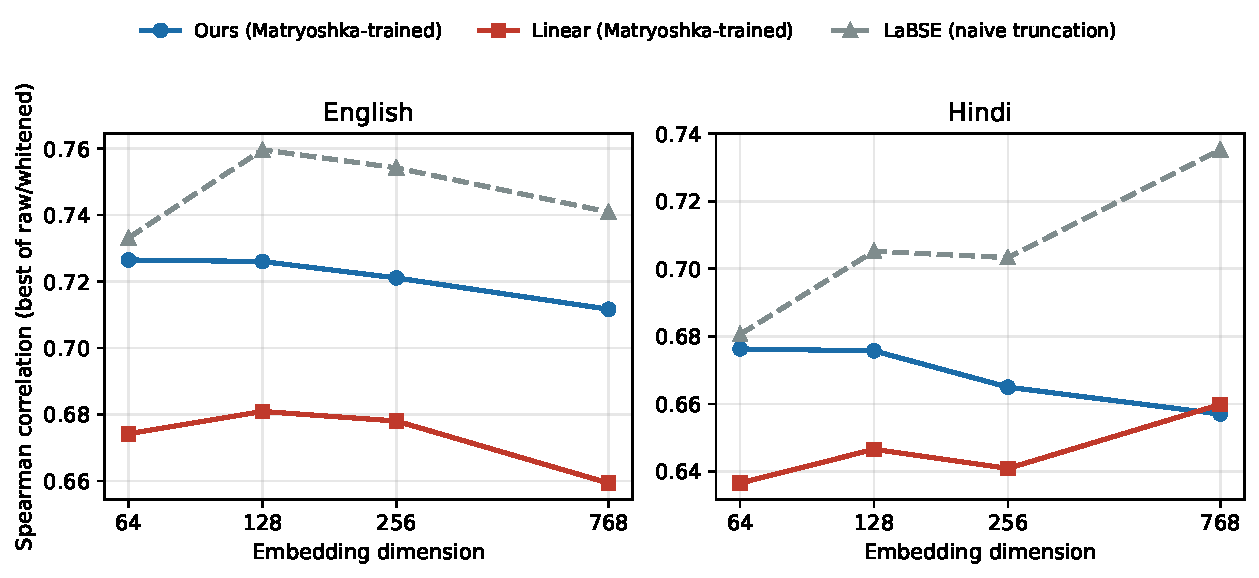
\includegraphics[width=\linewidth]{figures/matryoshka_curve.pdf}
\caption{Table~\ref{tab:matryoshka} plotted: accuracy versus embedding dimension for the structured head, the linear head, and naively-truncated LaBSE, both Matryoshka-trained heads flat to improving down to 64 dimensions while LaBSE's untrained truncation degrades, most visibly on Hindi.}
\Description{Two line charts, English and Hindi, plotting Spearman correlation against embedding dimension (64, 128, 256, 768, log scale) for three lines each: the Matryoshka-trained structured head and linear head both stay flat or rise slightly as dimension shrinks to 64, while naively-truncated LaBSE declines, most sharply in the Hindi panel.}
\label{fig:matryoshka-curve}
\end{figure}

For the structured head, compression is flat to slightly improving in every language tested (768$\to$64 dimensions): English $+0.0148$, Bangla $-0.0002$, Telugu $+0.0010$, Hindi $+0.0193$, Arabic $+0.0347$. This is evidence the accuracy-preserving property comes from the Matryoshka objective itself, not from truncation being harmless in general -- LaBSE's naive truncation, by contrast, degrades on Hindi. The linear head, trained through the identical Matryoshka recipe, does not share this property. English ($+0.0149$) and Telugu ($+0.0097$) still improve, but Bangla degrades ($-0.0173$), and Hindi ($-0.0233$) and Arabic ($-0.0433$) degrade more sharply -- Arabic's is the largest drop either head shows on any language. This is the one place in this study where the structured architecture shows a real, measured advantage: graceful compression under Matryoshka training is not automatic, and it does not transfer from one pooling head to another by default. The mechanism behind it is not something this paper's ablations isolate; we report it as an open finding, not an explained one.

\subsection{Fine-Tuned Baseline Comparison}
\label{sec:results:finetuned}

Every comparison above trains our architecture and compares it to LaBSE and mE5 used zero-shot. For English, we additionally fine-tune both baseline models under a reduced protocol: 300 STS-B pairs, 2 epochs, every parameter updated, evaluated on the full 1,379-pair test set.

\begin{table}[h]
\caption{Zero-shot versus reduced-protocol fine-tuned baselines, English STS-B.}
\label{tab:finetuned-baselines}
\begin{tabular}{@{}lrrrr@{}}
\toprule
Model & Params & Zero-shot & Fine-tuned (reduced) & $\Delta$ \\
\midrule
multilingual-E5-base & 278.0M & 0.8564 & 0.8551 & $-0.0013$ \\
LaBSE                 & 470.9M & 0.7154 & \textbf{0.7973} & $\mathbf{+0.0819}$ \\
\bottomrule
\end{tabular}
\end{table}

mE5's result is a genuine null finding. Its zero-shot representation is already near its own ceiling on English STS-B. LaBSE responds very differently. The same reduced protocol moves it $+0.0819$, to $0.7973$: $0.059$ above our own best English result, and $0.081$ above the linear head, despite training on the same 300 pairs for the same 2 epochs. So ``near-parity with LaBSE,'' wherever it is stated in this paper, refers specifically to LaBSE's zero-shot capability. Once allowed to fine-tune, LaBSE moves decisively ahead. Table~\ref{tab:all-english} assembles every method evaluated on English STS-B, same test set, into one ranking.

\begin{table}[h]
\caption{Every method evaluated on English STS-B, same test set and metric, ranked.}
\label{tab:all-english}
\begin{tabular}{@{}lrl@{}}
\toprule
Model & Spearman & Trained on our data \\
\midrule
multilingual-E5-base (zero-shot) & 0.8564 & No \\
multilingual-E5-base (fine-tuned, reduced) & 0.8551 & Yes \\
LaBSE (fine-tuned, reduced) & 0.7973 & Yes \\
\textbf{Structured head (Ours)} & \textbf{0.7383} & Yes \\
Linear head & 0.7164 & Yes \\
LaBSE (zero-shot) & 0.7154 & No \\
Untrained baseline (no head) & 0.6629 & No \\
\bottomrule
\end{tabular}
\end{table}

English is the one language where our specific mechanisms win the narrower comparison of Table~\ref{tab:baseline-head}. Even there, the full architecture places fourth of seven against every method this paper tested, behind both fine-tuned baselines and mE5's zero-shot number. Table~\ref{tab:baseline-head} asks whether attention-and-composition is worth its cost relative to the simplest structured alternative. Table~\ref{tab:all-english} asks where it stands against the strongest available options overall. Both answers are correct at the same time, and we report both: below every fine-tuned baseline tested, and below one baseline's zero-shot number entirely.

\subsection{Qualitative Examples}

We report five concrete cases, found by scanning test-set pairs for the clearest illustration of patterns already established quantitatively. We did not select them to overstate results. The untrained baseline assigns cosine similarity $0.975$ to the unrelated pair ``A person is boiling noodles.''/``A cat is licking a bottle.'' (gold $0.0$). Our trained embedding assigns $0.012$, correctly near zero. But for ``Rocky and Apollo Creed are running down the beach.''/``The men are jogging on the beach.'' (gold $0.6$), our model assigns only $0.259$, apparently failing coreference resolution, while LaBSE assigns $0.600$. A Bangla true-paraphrase pair, two headlines meaning ``Russia warns the European Union,'' scores $0.994$. A correctly-rejected near-miss, the same named individual in two different news events, scores $0.062$. On bitext retrieval, an English sentence's correct Bangla translation ranks third of eighty candidates before alignment training, and first of eighty after -- a smaller, separate 80-sentence pool built for this single illustrative example, not Table~\ref{tab:bitext}'s 500-sentence evaluation pool.

\section{Discussion and Limitations}
\label{sec:results:limitations}

\textbf{On the central finding.} Twenty-one of twenty-two controlled comparisons, across three task types and five languages, favor the linear head over the specific cognitively-motivated mechanisms this paper set out to justify -- this count is which head had the higher point estimate, not which margins are statistically established, and not twenty-two independent draws: every task-type comparison for a language reuses that language's same two trained heads (Statistical rigor, below, discusses both points in full). Only three of the five fair-baseline margins survive a significance test. Table~\ref{tab:comparison-count} lists exactly how these twenty-two decompose. A third qualification applies on top of the first two, and it is the largest of the three: all twenty-two comparisons are run at one fixed, untuned capacity that gives the structured head $7.5\times$ more trainable parameters than the linear head it is compared against. That capacity gap is itself a confound, not a neutral background condition, and we tested it directly rather than leaving it as a caveat: a parameter-matched control, run for four of the five languages, reverses the outcome robustly in Hindi, where the structured head beats the linear head outright, and only marginally, not confidently, in Arabic (Capacity as a confound, below). The twenty-one-of-twenty-two count is therefore a description of what this specific, capacity-mismatched configuration does, not a verdict on whether the underlying mechanisms are worth their complexity in general -- the second question is where this paper's evidence is most mixed, not settled. The rest of this section works through that evidence in full: why English is the one exception and what the capacity-matched control changes and does not change (below); the statistical and methodological checks behind every number above, including whitening protocol, significance testing, hyperparameter choice, and data-size sensitivity; a second, independently-designed architecture tested for convergent evidence; and the scope, reproducibility, and coverage limits of the study as a whole.

\begin{table}[h]
\caption{How the twenty-two comparisons decompose: task type, language, count, and how many favor the linear head.}
\label{tab:comparison-count}
\resizebox{\linewidth}{!}{%
\begin{tabular}{@{}llrr@{}}
\toprule
Task type & Languages & Comparisons & Favor linear head \\
\midrule
Similarity (Table~\ref{tab:baseline-head}) & English, Bangla, Telugu, Hindi, Arabic & 5 & 4 \\
Classifier transfer (Table~\ref{tab:classification}) & English (mono.); Bangla, Telugu, Arabic, Hindi (mono. + zero-shot) & 9 & 9 \\
Bitext retrieval (Table~\ref{tab:bitext}) & Bangla, Telugu, Hindi, Arabic, both directions & 8 & 8 \\
\midrule
Total & & 22 & 21 \\
\bottomrule
\end{tabular}%
}
\end{table} Section~\ref{sec:related-pooling} situates this within converging, independent evidence: Shen et al.~\citep{shen2018baseline}, Tang and Yang~\citep{tang2024poolingattention}, and Hara et al.~\citep{hara2026meanpooling} all show that structured pooling does not reliably earn its complexity over simple pooling on well-trained frozen representations. Task-conditioned pooling (Su et al.~\citep{su2022instructor}) is the established, mature answer to the deeper question of \emph{where} an embedding model should attend. It is not an open question this paper resolves. We regard this paper's value as the controlled, cross-lingual, cross-task demonstration of this pattern, for a specific, previously untested combination of mechanisms, reported honestly rather than as the positive result we expected going in.

\textbf{Why English is the exception.} The exception itself is not a single-benchmark artifact: the structured head wins five of seven English similarity benchmarks tested (Cross-benchmark generalization, below), so there is a real pattern to explain, not sampling noise from one test set. Beyond that, three pieces of evidence, not one experiment purpose-built to test this, converge on a data-availability explanation. First, English is the only language in this study with both a large native NLI pretraining corpus and a large native task-specific fine-tuning set; every other language relies on translated or cross-lingual transfer data, or skips task-specific fine-tuning entirely (Hindi, Arabic). Second, the component ablation (Table~\ref{tab:ablation}) shows the same pattern one level down: combining attention and composition helps in English and Bangla, the two languages with the most native fine-tuning data, and hurts in Telugu and Hindi, two of the three with the least. Third, the parameter-matched experiment (Capacity as a confound, below), run for four of the five languages under the leak-free protocol, offers real but mixed support for this pattern. Bangla, which has some native training data, shows a real but partial narrowing -- roughly two-thirds of the gap closes, not all of it -- consistent with the data-availability account. Telugu, which also has some native data, shows no narrowing at all, a data point that does not support the story. Hindi, which has no native task-specific data at all, shows a full, robust reversal -- the single strongest piece of evidence for this account anywhere in the paper. Arabic, also with no native task-specific data, shows a reversal too small to distinguish confidently from zero. Read plainly: of the two zero-native-data languages, one (Hindi) gives this account its strongest support and the other (Arabic) gives it only marginal, unconfirmed support; of the two some-native-data languages, only Bangla behaves as the account predicts, and Telugu does not. This is a real but partial confirmation of the data-availability account. We ran the direct test this argument needed: a data-size sweep holding each language fixed while training-data quantity varies (Data-size sensitivity, below). It partly confirms and partly complicates the story. All four non-English languages show the linear head's advantage shrinking as data grows, direct support for capacity earning its cost with more data -- Bangla's trend is nearly as clean as Hindi's and Telugu's, matching what the capacity-matched control above suggested it would be; Arabic's is the noisiest of the four (Data-size sensitivity, below). English does not show the mirror pattern either: the structured head's margin is already positive and roughly stable at just 10\% of its task-specific data, not growing the way the other languages' margins shrink. Because that sweep varied only task-specific data and held English's much larger NLI pretrain corpus fixed, it cannot separate two explanations: English needs comparatively little task data because its NLI pretraining already carries most of the advantage, or task-data quantity was never the operative variable for English specifically. Data availability remains the explanation most consistent with the paper's other patterns, but it is now a more precise, partially open question rather than a fully confirmed one.

\textbf{Capacity as a confound.} The structured head has $7.5\times$ more trainable parameters than the linear head, and both are trained under the same fixed recipe rather than one re-tuned per architecture. This leaves open whether the linear head wins because the cognitively-motivated mechanisms are unnecessary, or because the structured head is harder to optimize at this scale and never gets the chance to use its extra capacity. We tested this directly for all four non-English languages, under the same leak-free protocol as Table~\ref{tab:baseline-head}: a parameter-matched structured head ($K{=}2$ attention heads, GRU hidden size $52$, pre-combine bottleneck dimension $104$ -- the same attention-and-composition-and-combine design, scaled down rather than changed) reaches $589{,}280$ trainable parameters, within $0.2\%$ of the linear head's $590{,}592$, identically across all four.

Bangla is robust to the correction. Matched capacity reaches $0.8582$ (raw; dev-fit whitening does not help here either, $0.8862$), beating its own full-capacity structured head ($0.8452$) by $+0.0130$ -- direct evidence the extra capacity was actively hurting, not simply idle. It still trails the linear head ($0.8647$) by $-0.0065$, down from $-0.0194$ at full capacity: the gap narrows by roughly two-thirds but does not close.

Telugu is not. Under the original protocol, Telugu's matched-capacity head appeared to narrow its gap to linear from $-0.0144$ to $-0.0119$, a modest closing, echoing Bangla on a smaller scale. Under the corrected, leak-free protocol, that narrowing disappears entirely: matched capacity reaches $0.7758$, which is $-0.0010$ \emph{below} its own full-capacity structured head ($0.7768$), not above it, and trails the linear head ($0.7912$) by $-0.0154$ -- slightly \emph{wider} than the full-capacity gap of $-0.0144$, not narrower. Telugu's dev split is small ($n{=}130$) and its dev-fit-whitened score is far worse than raw ($0.6848$ vs.\ $0.7758$), so this reversal-of-a-direction is plausibly noise from a small, ungenerous dev fit rather than a real change in the underlying effect -- but we report the number the corrected protocol actually gives, not the more flattering one it replaces.

Hindi and Arabic initially appeared as a matched pair: both reverse the full-capacity result, not just narrow it. That pairing does not hold evenly. Hindi's matched-capacity structured head reaches $0.7313$ (raw; dev-fit whitening does not help here either, $0.6859$), beating its own full-capacity structured head ($0.6777$) by $+0.0536$ and beating the linear head ($0.7061$) by $+0.0252$, unchanged from the pre-correction estimate, against a full-capacity gap of $-0.0283$. Arabic's reversal survives in sign only. Matched capacity reaches $0.4573$ (raw; dev-fit whitening actively hurts here, $0.3907$, on a dev split of just $n{=}32$), beating full capacity ($0.4149$) by $+0.0424$, but beating the linear head ($0.4526$) by only $+0.0047$ -- roughly a third of the already-small effect it needs to be distinguishable from zero, and an order of magnitude smaller than the pre-correction estimate ($+0.0156$). We do not treat this as a confidently-established reversal: it has no formal significance test of its own (Statistical rigor, above, covers the full-capacity fair-baseline margins, not this capacity-matched follow-up), and a margin this close to zero, on a dev split of 32 examples, is not evidence we would trust without one.

This picture is more mixed than a single pass would suggest: capacity mismatch convincingly explains part of Bangla's margin and the entirety of Hindi's reversal; Arabic's reversal is real in sign but too small to lean on without further testing; and Telugu shows no narrowing at all. \textbf{Capacity is a substantial confound in this comparison, but its effect is language-dependent, not global: it fully explains Hindi's reversal, partially explains Bangla's margin, is too weak to establish in Arabic without further testing, and does not explain Telugu's margin at all.} This qualifies, rather than reverses, the paper's central complication: the structured head's failure to earn its complexity at full capacity is still not simply "the mechanisms are unnecessary" in at least Hindi's case, but the evidence for that claim generalizing further than Hindi is weak, and readers should weight the Hindi result accordingly rather than treat all four languages as equally supportive. We also ran the other lever raised in Section~\ref{sec:experiments}'s small-batch confound: a batch-size sweep for Bangla, both heads, at 32, 64, and 128, under the same leak-free protocol as the primary tables, with raw scoring throughout for both heads (Whitening leakage, above). The gap narrows sharply from batch 32 to 64 (ours: $0.8452\to0.8768$; linear: $0.8647\to0.8792$; gap: $-0.0194\to-0.0024$) but widens back out at 128 (ours: $0.8688$; linear: $0.8840$; gap: $-0.0153$) -- not a clean trend in either direction. Batch 64's near-zero gap is a weak point in favor of the capacity-confound hypothesis, but batch 128 widening back out means more negatives do not decisively and consistently favor the structured head across this sweep. Techniques from the broader contrastive-learning-stability literature are natural candidates for testing the residual gap further: representation-rank dynamics during fine-tuning~\citep{jung2024rank} and hard-negative-focused reweighting of the InfoNCE objective~\citep{hou2023focalinfonce} both target exactly the small-batch, low-resource optimization regime this study operates in, though neither was applied here. Expected effects, if they were: at batch size 32, most in-batch negatives are easy (unrelated sentences), so focal reweighting should sharpen the gradient signal from the few hard negatives present; we would expect this to matter more for the structured head, which has more parameters and more room to fit noise from a diluted signal, than for the linear head. Rank-dynamics control speaks more directly to the optimization-difficulty hypothesis itself: if the structured head's representation rank behaves differently during fine-tuning than the linear head's, that would be direct evidence for "harder to optimize" rather than "mechanism unnecessary." Neither expectation is tested here.

\textbf{Memory evaluation scale.} The scoring-variant comparison (Table~\ref{tab:memory-variants}) that favors content-only scoring rests on a single English discourse-retrieval split: 257 query items, only 181 for training. This is enough to show that CoALA-inspired scoring overfits its 984,577 parameters at this scale -- the train/validation AUROC gap in Section~\ref{sec:results:memory} makes that clear -- but it is not enough to conclude content-only scoring is optimal at any scale. A larger training set could let the learned variants earn their capacity. Our recommendation is a practical default under this study's compute and data budget, not evidence that scoring complexity never helps memory-aware retrieval.

\textbf{Whitening leakage.} Whitening is fit only on each language's held-out dev split, never the test set (Section~\ref{sec:experiments}): for every language and both heads, whitening is fit on that language's dev split (English: STS-B validation, $n{=}500$; Bangla: BnPC validation, $n{=}500$; Telugu: SemRel dev, $n{=}130$; Hindi: SemRel dev, $n{=}288$, unused elsewhere in training; Arabic: SemRel dev, $n{=}32$, also unused elsewhere), and Table~\ref{tab:specialist} and Table~\ref{tab:baseline-head} report this leak-free selection as the paper's primary numbers. The winning head is identical under the earlier, leaky test-fit protocol in all five languages -- English still favors the structured head, Bangla/Telugu/Hindi/Arabic still favor the linear head -- so leakage does not explain this study's central result. Leak-free scoring changes the exact numbers, not the qualitative pattern, with one exception: Hindi's structured head falls below its own untrained baseline, obscured under test-fit whitening by a leakage-specific boost (Arabic and Hindi, above).

Raw scoring outperforms dev-fit whitening in all five languages under a properly leak-free selection rule. An earlier version of Table~\ref{tab:specialist} and Table~\ref{tab:baseline-head} selected dev-fit whitening for Bangla because it scored higher on the \emph{test} set specifically -- comparing two candidate scoring methods on test and reporting the winner, a mild form of test-set peeking distinct from (and left uncaught by) the whitening-fit leakage this correction otherwise addresses. A held-out check settles it: fit whitening on one random half of Bangla's dev split, decide raw-vs-whitened on the other half, and never touch test at all. Whitening loses decisively on that held-out half (AUROC $0.84$ raw vs.\ $0.69$ whitened for both heads, not a close call), so Table~\ref{tab:specialist} and Table~\ref{tab:baseline-head} now report Bangla's raw score throughout, matching the other four languages, where raw already won on both dev and test. This changes Bangla's absolute numbers substantially (structured: $0.8732\to0.8452$; linear: $0.8926\to0.8647$) but its margin barely at all ($-0.0194$ either way), since the same selection procedure applied to both heads.

Every extended analysis in this paper now uses this same leak-free protocol: the parameter-matched capacity experiments (Capacity as a confound, below), the batch-size sweep (also below), the multi-seed grid (Table~\ref{tab:multiseed-fair-baseline}), the data-size sweep (Table~\ref{tab:data-size}, below), the layer-wise attention comparison (Table~\ref{tab:layer-attn}, below), the Arabic Farasa experiment (Arabic and Hindi, below), the bootstrap significance test, and the English cross-benchmark STS suite (Table~\ref{tab:sts-suite}, below). Correcting each in turn changed exact numbers throughout, and in several places changed which conclusion the analysis itself supports, not just its precision: the capacity-matched control's Telugu and Arabic results (Capacity as a confound, below); the multi-seed grid's Hindi result, which now agrees with the bootstrap rather than appearing to contradict it (Statistical rigor, below); and the data-size sweep's Hindi result, which now shows the same clean shrinking trend Telugu and Bangla show (Data-size sensitivity, below). Bangla required one further check, distinct from the whitening-fit leakage above: choosing raw versus whitened by which scores higher on the test set is itself a mild form of test-set peeking. A held-out check (whitening fit on one half of Bangla's dev split, the choice decided on the other half, test never touched) confirms raw is the right choice for Bangla too, matching the other four languages; every Bangla number in this paper uses raw scoring. The margin this reflects is nearly identical either way, since the same selection procedure applies to both heads, though the absolute numbers move more. Each correction is discussed where it is used rather than summarized here; none reverses this paper's central comparison.

\textbf{Cognitive validity.} None of this is evidence that the resulting embeddings are cognitively valid, in the sense of matching human behavioral data. We have not collected human similarity judgments or reaction-time data. ``Cognitively-motivated'' describes the mechanisms' inspiration here, not a validated property.

\textbf{Statistical rigor.} The shared-backbone configuration (Table~\ref{tab:multiseed}) was, until this analysis, the only multi-seed check in the paper. We ran a paired bootstrap significance test for every language in the fair-baseline comparison (Table~\ref{tab:baseline-head}), under the same leak-free evaluation protocol now used as primary throughout that table (whitening fit on development data where evaluated; raw wins for both heads in every language, Whitening leakage, above): 10,000 resamples of the test set, with the raw-vs-whitened choice fixed to match each cell's published number rather than re-selected per resample, which would bias the result. Three of five margins are statistically significant at $\alpha=0.05$: English ($+0.0219$, 95\% CI $[+0.0013, +0.0432]$, favoring the structured head), Bangla ($-0.0194$, 95\% CI $[-0.0329, -0.0064]$, favoring the linear head), and Hindi ($-0.0283$, 95\% CI $[-0.0550, -0.0010]$, $n=968$, favoring the linear head). The other two point the same direction as their point estimates but are not statistically distinguishable from zero at this study's sample sizes: Telugu ($-0.0144$, 95\% CI $[-0.0450, +0.0166]$, $n=297$) and Arabic ($-0.0377$, 95\% CI $[-0.0965, +0.0190]$, $n=595$). Read plainly: the linear head's advantage is statistically established in two languages (Bangla, Hindi) and statistically absent in one (English, where the structured head wins instead); in the remaining two, the point estimates favor the linear head but the sample is too small to rule out no difference at all. Hindi's significance reflects the leak-free correction, which removed a whitening boost specific to Hindi's structured head (Whitening leakage, above) and widened the margin -- the opposite of what an artifact of that correction would predict, evidence the effect is real rather than noise. Table~\ref{tab:multiseed-fair-baseline}'s multi-seed retraining below, also computed under the leak-free protocol, agrees: Hindi's linear-favoring margin is stable across all three independently-trained seeds, not only across bootstrap resamples of one trained model -- two different sources of uncertainty (training-run variance and test-set resampling) pointing the same direction. The twenty-one-of-twenty-two count reported throughout this paper describes which head scored higher, not which margins are statistically established -- a distinction this analysis draws for the first time here.

We additionally retrained both heads at two more seeds (123, 2024) for every language in the fair-baseline comparison, under the same leak-free protocol as the primary tables, extending true multi-seed retraining beyond the shared-backbone configuration for the first time (Table~\ref{tab:multiseed-fair-baseline}). This is a different source of uncertainty than the bootstrap above -- test-set resampling holds the trained model fixed and asks how stable its score is, while multi-seed retraining asks how stable the training itself is -- and the two do not always agree. English and Bangla confirm the bootstrap: the same head wins at all three seeds, with non-overlapping ranges (English $[0.7383,0.7474]$ vs.\ $[0.7164,0.7247]$; Bangla $[0.8413,0.8452]$ vs.\ $[0.8647,0.8825]$). Telugu and Hindi also now confirm the bootstrap: the linear head wins at all three independently-trained seeds in both, with non-overlapping ranges (Telugu $[0.7506,0.7768]$ vs.\ $[0.7912,0.8025]$; Hindi $[0.6777,0.6979]$ vs.\ $[0.7061,0.7119]$) -- for Telugu, this is evidence the single-seed bootstrap could not see on its own, since it cannot detect a systematic effect of training itself, and for Hindi it is a second, independent confirmation of the bootstrap's significant margin. Arabic is the one language where the two sources of uncertainty still diverge: the structured head's standard deviation ($0.0268$) is roughly $3.9\times$ the linear head's ($0.0069$), with scores spanning $0.3803$ to $0.4460$ across seeds -- a swing of $0.0657$ from random initialization alone, on the one language already flagged as anomalous (Arabic, below), and the linear head wins only two of the three seeds. This remains the clearest direct evidence in this study that the structured head is harder to optimize at this scale, not just unnecessary.

We ran the same test on classifier transfer (Table~\ref{tab:classification}): the classifier fit is held fixed and the test set is bootstrap-resampled, since accuracy only depends on the (unresampled) training embeddings through a fixed classifier. All nine accuracy margins are significant, all favoring the linear head: English monolingual ($-0.0653$, 95\% CI $[-0.0807, -0.0504]$), Bangla monolingual ($-0.0798$, CI $[-0.0965, -0.0636]$) and zero-shot ($-0.1164$, CI $[-0.1355, -0.0982]$), Telugu monolingual ($-0.0548$, CI $[-0.0713, -0.0387]$) and zero-shot ($-0.0609$, CI $[-0.0790, -0.0427]$), Arabic monolingual ($-0.0587$, CI $[-0.0743, -0.0430]$) and zero-shot ($-0.0592$, CI $[-0.0773, -0.0410]$), and Hindi monolingual ($-0.0501$, CI $[-0.0656, -0.0346]$) and zero-shot ($-0.1040$, CI $[-0.1227, -0.0851]$). Macro-F1 margins are significant in the same direction for all nine as well -- English $-0.0717$, CI $[-0.0957,-0.0481]$; Bangla $-0.0763$/$-0.0855$ (mono/zero-shot); Telugu $-0.0697$/$-0.0551$; Arabic $-0.0728$/$-0.0460$; Hindi $-0.0655$/$-0.0916$ -- confirming the accuracy pattern is not an artifact of averaging over MASSIVE's imbalanced classes. Classifier transfer is where this paper's linear-head result is most statistically robust, on both metrics; the fair-baseline similarity comparison above is where it is weakest. (A training-data class-coverage bug, since fixed (Section~\ref{sec:results:classification}), had made Hindi monolingual appear as a near-tie rather than significant; that near-tie was an artifact of the bug, not a property of the embeddings.) Bitext-retrieval comparisons remain single runs, with no formal significance test. The predictive head's initial weights are not seed-pinned, so its exact Recall@$k$ values vary between runs, though the qualitative pattern does not.

One further caveat applies to the twenty-two-comparison count itself (Table~\ref{tab:comparison-count}): the twenty-two are not twenty-two independent draws. Every task-type comparison for a given language reuses that language's same two trained heads, so a language-level effect -- backbone quality, data availability, whatever drives Bangla's or English's overall pattern -- pushes several of the twenty-two in the same direction at once. Treating each of the twenty-two as independent, as the raw count implicitly does, likely overstates how much independent evidence twenty-one-of-twenty-two actually represents; the per-language, per-task significance tests above are the more honest unit of evidence than the count.

\textbf{Arabic and Hindi.} Training with AraBERT underperforms its own untrained baseline. Under the leak-free protocol now used throughout (Table~\ref{tab:baseline-head}), Hindi shows the same pattern, obscured under leaky test-fit whitening by a boost specific to Hindi's test set (Table~\ref{tab:baseline-head}, above). Arabic is the more severe and better-understood case; the rest of this discussion focuses there, though the caution about capacity and instability below applies to Hindi's much smaller gap as well. We rule out two candidate causes directly for Arabic. Truncation: Arabic sentences average 15.9 tokens, and only $0.3\%$ are truncated. Raw anisotropy: Arabic's score of $0.5694$ is the best-conditioned of all five languages, not the worst. We tested a third candidate directly: missing Farasa preprocessing, recommended by AraBERT's own documentation but not applied to any of this paper's main results. Re-running Arabic end to end with Farasa segmentation and AraBERT's normalization applied to every sentence (XNLI training triplets and SemRel test pairs alike), and scored under the same leak-free evaluation protocol as Table~\ref{tab:baseline-head} (whitening fit on development data where evaluated), lifts every score substantially over the non-Farasa leak-free numbers: untrained baseline $0.4498\to0.5943$ ($+0.1445$), linear head $0.4526\to0.5711$ ($+0.1185$), structured head $0.4149\to0.5563$ ($+0.1414$), gains of roughly $12$ to $14$ Spearman points. Farasa preprocessing is clearly the right choice for AraBERT in an absolute sense, and this paper's main Arabic numbers understate what the backbone can do. The structured-head anomaly survives this correction too, and slightly sharpens: the Farasa-preprocessed structured head ($0.5563$) still trails its own Farasa-preprocessed untrained baseline ($0.5943$) by $-0.0380$ (vs.\ $-0.0267$ under leaky test-fit whitening). One genuinely new wrinkle appears under leak-free scoring: the linear head now also falls below the untrained baseline ($0.5711$ vs.\ $0.5943$, $-0.0232$), where it had cleared it easily under the leaky protocol ($0.5801$ vs.\ $0.5545$, $+0.0256$). We do not read this as the linear head suddenly sharing the structured head's problem: on raw cosine similarity alone, with no whitening at all, both heads still beat the untrained baseline cleanly (structured $0.5153$, linear $0.5510$, untrained $0.5033$), and the reversal appears only once whitening is fit on Arabic's $32$-example dev split specifically -- a transform estimated from 32 pairs is a noisy statistic, and it is plausible this particular fit happens to flatter the untrained baseline's test score by chance. The structured-head anomaly, by contrast, is robust to the protocol correction and, if anything, larger under it; the linear-vs-untrained comparison is not clean, and we do not treat it as established either way pending further testing -- but preprocessing does not explain why training the structured head specifically makes things worse. Two candidates remain plausible but unconfirmed: weaker signal in the translated training data, and an eval-domain mismatch between translated-NLI training and native SemRel2024 evaluation, which Hindi now shares in outcome as well as setup. A fourth candidate now has direct support: training instability itself. Arabic's multi-seed standard deviation for the structured head ($0.0268$, Statistical rigor above) is more than double any other language's, so at least part of what looks like an architecture failure may be this specific language-backbone pairing's optimization landscape, not the mechanisms themselves -- and with Farasa now ruled out, this is the strongest remaining candidate.

\textbf{Hyperparameters.} $K=4$ attention heads and GRU size $m=128$ were fixed at literature precedent, not tuned. The joint three-language ablation (Table~\ref{tab:ablation}) already costs 6{,}824s per run. We tested one specific point on this space directly -- the parameter-matched structured head above, $K{=}2$, $m{=}52$ -- rather than a full sweep; a broader sweep across intermediate $(K,m)$ values, for the other four languages, remains untested.

\textbf{Data-size sensitivity.} We ran the direct test: 10\%/25\%/50\%/100\% of each language's available training data, both heads, holding the language fixed while data quantity varies, under the same leak-free protocol as the primary tables (Table~\ref{tab:data-size}). English and Bangla vary task-specific fine-tuning data, with English's NLI pretrain corpus held at full size throughout, since that stage has no per-language equivalent to scale against; Hindi and Arabic, which have no task-specific data at all, vary XNLI pretrain-triplet count instead. All four non-English languages support the capacity hypothesis, though not equally cleanly. Telugu's linear-favoring margin shrinks steadily across every step ($-0.0597\to-0.0144$). Hindi's does too as XNLI pretrain data grows ($-0.0681\to-0.0267$), essentially flat from 50\% to 100\%. Bangla's follows nearly the same shape as task data grows ($-0.0490\to-0.0187$), also essentially flat from 50\% to 100\% ($-0.0194$). Arabic is the noisiest of the four: its margin shrinks from 25\% to 50\% of its NLI data ($-0.0782\to-0.0224$) before widening again at 100\% ($-0.0377$) -- consistent with, not contradicting, the high seed-to-seed variance already documented for Arabic's structured head (Statistical rigor, above), since the 100\% point is a single run within that noisy distribution. English complicates the story instead of confirming it: the structured head's margin is positive throughout but does not grow with data the way the other languages' margins shrink ($+0.0329$ at 10\%, $+0.0219$ at 100\%, no clear trend in between). Since only task data was varied for English, this sweep cannot distinguish "English needs less task data because its NLI pretrain corpus already does the work" from "task-data quantity is not actually what drives English's exception." That distinction remains the more precise open question, not simply whether more data would flip the other languages -- all four non-English languages suggest it eventually would, Arabic least cleanly; English suggests data quantity alone is not the whole story even there.

\begin{table}[h]
\caption{Data-size sensitivity: linear-vs-structured margin (ours $-$ linear) at 10\%/25\%/50\%/100\% of each language's training data, under the same leak-free protocol as Table~\ref{tab:baseline-head}. English/Bangla/Telugu vary task-specific data; Hindi/Arabic vary NLI pretrain-triplet count (no task-specific data exists for either).}
\label{tab:data-size}
\begin{tabular}{@{}lrrrr@{}}
\toprule
Language & 10\% & 25\% & 50\% & 100\% \\
\midrule
English & $+0.0329$ & $+0.0132$ & $+0.0234$ & $+0.0219$ \\
Bangla  & $-0.0490$ & $-0.0342$ & $-0.0187$ & $-0.0194$ \\
Telugu  & $-0.0597$ & $-0.0530$ & $-0.0291$ & $-0.0144$ \\
Hindi   & $-0.0681$ & $-0.0670$ & $-0.0267$ & $-0.0283$ \\
Arabic  & $-0.0776$ & $-0.0782$ & $-0.0224$ & $-0.0377$ \\
\bottomrule
\end{tabular}
\end{table}

\textbf{A third pooling strategy: layer-wise attention.} Layer-wise attention pooling over the frozen encoder's hidden layers~\citep{oh2022dontjudge} sits between the two heads compared throughout this paper: a learned multiplicative attention over each layer's representation, concatenated with the last layer's [CLS] token, through an MLP ($3{,}540{,}480$ trainable parameters -- more than the linear head's $590{,}592$, less than the structured head's $4{,}430{,}592$). We implemented it exactly (Equations 1-5 of the cited paper) and ran it through the same fair-baseline protocol, all five languages, same data, same recipe, under the same leak-free evaluation protocol as Table~\ref{tab:baseline-head} (whitening fit on development data where evaluated). It never wins. In every language, both the linear head and the structured head outrank it: English ($0.7383$ structured, $0.7164$ linear, $0.7144$ layer-attn), Bangla ($0.8647$ linear, $0.8452$ structured, $0.8300$ layer-attn), Telugu ($0.7912$ linear, $0.7768$ structured, $0.7188$ layer-attn). Layer-wise attention pooling falls below the untrained baseline in three of five languages, not just the two zero-shot, XNLI-pretrain-only ones: Hindi ($0.6581$ vs.\ $0.6908$ untrained) and Arabic ($0.4024$ vs.\ $0.4498$ untrained) by a wide margin as before, and now Telugu too, by a narrow one ($0.7188$ vs.\ $0.7213$ untrained) -- a language with some native task-specific data, not a zero-shot setting, joining the pattern only once whitening leakage is corrected. Training this specific architecture actively hurts in three of five languages, more severely than either head tested elsewhere in this paper. A third, independently-published structured pooling mechanism failing to beat the simplest baseline, using a completely different attention formulation (layers, not tokens or composition), is independent evidence for this paper's central pattern, not a repetition of it.

\begin{table}[h]
\caption{Layer-wise attention pooling~\citep{oh2022dontjudge} against the untrained baseline, linear head, and structured head, all five languages, under the same leak-free evaluation protocol as Table~\ref{tab:baseline-head} (whitening fit on development data where evaluated).}
\label{tab:layer-attn}
\begin{tabular}{@{}lrrrrl@{}}
\toprule
Language & Untrained & Layer-attn & Linear & Structured & Rank of layer-attn \\
\midrule
English & 0.6629 & 0.7144 & 0.7164 & \textbf{0.7383} & 3rd of 4 \\
Bangla  & 0.6591 & 0.8300 & \textbf{0.8647} & 0.8452 & 3rd of 4 \\
Telugu  & 0.7213 & 0.7188 & \textbf{0.7912} & 0.7768 & 4th of 4 \\
Hindi   & 0.6908 & 0.6581 & \textbf{0.7061} & 0.6777 & 4th of 4 \\
Arabic  & 0.4498 & 0.4024 & \textbf{0.4526} & 0.4149 & 4th of 4 \\
\bottomrule
\end{tabular}
\end{table}

\textbf{Cross-benchmark generalization of the English exception.} English similarity elsewhere in this paper is measured on STS-B only. We tested whether the structured head's win generalizes, using the same trained checkpoints (no retraining), on the full standard STS suite: STS12, STS13, STS14, STS15, STS16, and SICK-R, scored under the same leak-free evaluation protocol as Table~\ref{tab:baseline-head} (whitening fit on STS-B validation, English's development split). Table~\ref{tab:sts-suite} reports each benchmark separately rather than only the aggregate five-of-seven pattern, since an average or a win-count alone would hide that the two losses are not evenly spread across benchmark sizes or scores.

\begin{table}[h]
\caption{English STS suite, per-benchmark Spearman $\rho$ (best of raw/dev-fit-whitened per head, leak-free). Same trained checkpoints as Table~\ref{tab:baseline-head}, no retraining.}
\label{tab:sts-suite}
\begin{tabular}{@{}lrrrrl@{}}
\toprule
Benchmark & $n$ & Ours & Linear & Margin (Ours$-$Linear) & Winner \\
\midrule
STS-B  & 1{,}379 & 0.7383 & 0.7164 & $+0.0219$ & Ours \\
STS12  & 3{,}108 & 0.6710 & 0.5921 & $+0.0789$ & Ours \\
STS13  & 1{,}500 & 0.7304 & 0.7214 & $+0.0090$ & Ours \\
STS14  & 3{,}750 & 0.6575 & 0.6365 & $+0.0211$ & Ours \\
STS15  & 3{,}000 & 0.7542 & 0.7865 & $-0.0322$ & Linear \\
STS16  & 1{,}186 & 0.7535 & 0.7180 & $+0.0355$ & Ours \\
SICK-R & 9{,}927 & 0.7079 & 0.7195 & $-0.0117$ & Linear \\
\bottomrule
\end{tabular}
\end{table}

The winner pattern held under both whitening protocols -- the same five benchmarks (STS12, STS13, STS14, STS16, STS-B) favor the structured head and the same two (STS15, SICK-R) favor linear -- though individual margins shift substantially: STS12's margin more than doubles ($+0.0325\to+0.0789$), while STS13 and STS14's shrink to a fraction of their prior size ($+0.0298\to+0.0090$ and $+0.0460\to+0.0211$). That the winner pattern survives a protocol change large enough to move individual margins by a factor of three is evidence the five-of-seven result is not a leakage artifact.

The structured head wins five of seven English similarity benchmarks including STS-B; STS15 and SICK-R favor the linear head instead. This is not a single-benchmark artifact -- the exception is a majority pattern across seven independent test sets, not one lucky number -- but it is not universal, and it is not simply large test sets outvoting small ones: SICK-R is the suite's largest benchmark (n=9,927) and has one of the smallest margins ($-0.0117$), while the five wins span sample sizes up to 3,750 (STS14), larger than STS15's own 3,000. We have no explanation for why STS15 and SICK-R specifically break the pattern; testing that is future work. One caveat applies to this comparison specifically, and to English's NLI pretraining more generally: the evaluated checkpoint was pretrained on SNLI, whose premises are Flickr30k image captions~\citep{bowman2015snli}, while SICK-R is built in part from Flickr8k image captions and STS-2012 video-description pairs~\citep{marelli2014sick}, and STS14 includes an ``images'' subtask drawn from PASCAL VOC-2008 captions. These are different specific photo and caption pools than Flickr30k, so exact-sentence duplication between SNLI and these test sets is unlikely, but all of them are short, crowd-sourced image- or video-caption sentences from the same research era, a genre where near-duplicate or template-similar sentences recur across corpora even without a shared source image. We did not check for this directly, so part of this generalization result -- and, by the same logic, any English result downstream of the SNLI-pretrained checkpoint -- may not be as fully out-of-domain as an unrelated test set would be.

\textbf{Reproducibility.} All code, training and evaluation scripts, and run logs are available at \url{https://github.com/hasanoic/CognitiveEmbedding}. So are the JSON result tables behind every number in this paper. Every hyperparameter is a module-level constant in its script, not a separate configuration file. All experiments were run on Windows 10 (build 10.0.19045) with Python 3.11.9, PyTorch 2.13.0, Hugging Face Transformers 4.57.6, \texttt{datasets} 5.0.1, \texttt{huggingface\_hub} 0.36.2, sentence-transformers 3.4.1, scikit-learn 1.5.0, SciPy 1.17.1, NumPy 2.4.6, and pandas 3.0.5; the Farasa-preprocessed Arabic evaluation (Section~\ref{sec:results:limitations}) additionally used \texttt{farasapy} 0.1.1 and \texttt{arabert} 1.0.1. Exact package versions are also pinned in \texttt{requirements.txt} in the repository above.

\textbf{Baseline scope.} This paper's baselines are the ones the fair-baseline protocol itself requires: an untrained mean-pooled backbone, LaBSE, and multilingual-E5, each evaluated zero-shot and, for English, also fine-tuned (Section~\ref{sec:results:finetuned}). We do not compare against LASER3~\citep{heffernan2022laser3}, a strong bitext-mining-specific baseline, or against IndicBERT and MuRIL, language-specific encoders for Hindi and Telugu with no small-head fair-baseline protocol of their own to compare into. BGE-M3, cited in the Introduction as one of the strongest available pretrained models, is not run as an empirical baseline here either. Each would answer a different question -- how competitive is this study's frozen-encoder-plus-head approach against the current state of the art in absolute terms -- than the one this paper asks, which is whether a specific structured mechanism earns its cost over the simplest trained alternative, holding the backbone fixed. Both questions are legitimate; only the second is this paper's scope.

\textbf{Bitext retrieval pool construction.} The 500-sentence candidate pool (Table~\ref{tab:bitext}) is the first 500 rows of FLORES-200 devtest's on-disk order, not a random sample, capped from the full 1,012 to bound the retrieval step's $O(n^2)$ pairwise-similarity cost. FLORES-200's devtest sentences are grouped by source document and drawn from three domains -- Wikinews, WikiJunior, WikiVoyage -- in roughly equal proportion across the full corpus~\citep{nllbteam2022flores200}, but the \texttt{mteb/flores} mirror used here carries no domain or document metadata, so we cannot confirm this fixed truncation is domain-representative rather than skewed toward whichever domain appears first in the file. Alignment training draws its signal from the separate \texttt{dev} split instead: for each of the four non-English languages, all 997 English-X row-aligned pairs are loaded from \texttt{dev}, shuffled once with a fixed seed (\texttt{RANDOM\_SEED}$=42$), and split 88/12 into $878$ training pairs and $119$ held out for early stopping, identically for both heads. FLORES-200's 3,001 sentences are partitioned by the dataset's own creators into three non-overlapping splits -- \texttt{dev} (997), \texttt{devtest} (1,012), and a held-out \texttt{test} (992)~\citep{nllbteam2022flores200} -- so \texttt{dev} and \texttt{devtest} share no sentence by construction: no training pair and no candidate sentence are the same row, in any language.

\textbf{Language-set coverage across tasks.} Classifier transfer (Table~\ref{tab:classification}) covers English, Bangla, Telugu, Hindi, and Arabic; bitext retrieval (Table~\ref{tab:bitext}) covers Bangla, Telugu, Hindi, and Arabic, with English as the pivot language rather than a retrieval target -- a design property of the bitext-retrieval protocol, not a gap in scope. The two tasks therefore share full overlap on all four non-English languages, and the dissociation reported in Cross-Lingual Generalization (Section~\ref{sec:results:crosslingual}) is evidenced on all four jointly. MASSIVE~\citep{fitzgerald2022massive} supports Telugu (\texttt{te}) with the same 59-way intent taxonomy and 2,974-example test set as every other language, via the same mirror (\texttt{mteb/amazon\_massive\_intent}) this project loads from; Telugu's classifier-transfer results add two comparisons (monolingual and zero-shot), both significantly favoring the linear head, consistent with every other language tested.

\section{Broader Impact and Ethical Considerations}

This paper's practical contribution -- evidence that a linear projection is usually enough at the capacity this study tested, that capacity is a substantial confound in that result whose effect is language-dependent rather than uniform, and a protocol for checking both before building a more complex mechanism at all -- is aimed at researchers and practitioners with limited compute, which describes most work on Bangla, Telugu, Hindi, and Arabic sentence embeddings today. Recommending against unnecessary architectural complexity has a direct resource-saving effect for exactly the communities TALLIP serves. The fair-baseline protocol itself is reusable for any pooling mechanism, in any language, before publication.

The main limitation with broader-impact implications is encoder dependence: every result here is tied to one specialist backbone per language (Table~\ref{tab:data}), not tested against alternative pretrained encoders for the same language. A practitioner adopting this paper's linear-head recommendation should verify it holds for their specific backbone, not assume it transfers automatically. All datasets used are publicly released research corpora with documented provenance (BnPC, SemRel2024, MASSIVE, FLORES-200, XNLI, SNLI/MultiNLI, STS-B) or standard pretraining corpora for the cited backbone models; we did not construct new data collection from human subjects, so no new consent or annotation-labor considerations arise beyond what each cited dataset's own release already documents. None of these corpora were built by mining raw, unfiltered web text for parallel or similarity pairs -- unlike bitext-mining corpora assembled that way, each is a curated benchmark with its own published construction and quality-control process, which is the more relevant safeguard here than a separate offensive-content audit on our part.

\textbf{Conflict of interest.} The author declares no conflict of interest.

\section{Conclusion}

This paper set out to test whether four mechanisms motivated by human sentence processing are worth their complexity: attention and composition, which form the core embedding, and memory and prediction, evaluated as separate downstream capabilities. We tested them against the simplest possible alternative, under an identical, controlled protocol, across five typologically diverse languages and three task types. The strongest defensible conclusion is this: for the frozen encoders, datasets, training recipe, and evaluation tasks studied here, at the one fixed and untuned capacity configuration evaluated throughout ($7.5\times$ more trainable parameters than the linear head, $2.7$--$2.8\times$ slower training), the structured attention-plus-BiGRU head does not consistently outperform an identically trained linear projection. That capacity qualifier is load-bearing, not boilerplate: a parameter-matched control (Capacity as a confound, below), under the same leak-free protocol as the primary tables, reverses this outcome robustly in Hindi -- arguably the single most scientifically interesting result in this paper, since it shows the same mechanisms this paper otherwise reports as losing can win outright once a confound the rest of the comparisons do not control for is removed -- and only marginally, not confidently, in a second language (Arabic). Put more carefully than a raw count allows: across twenty-two task-language comparisons, the linear head has the higher point estimate in twenty-one; these are not twenty-two independent draws (Statistical rigor, below), and a formal significance test supports only a subset of them. The one exception, English semantic similarity, is also the single best-resourced setting in this study.

This is a narrower claim than ``structured or cognitively-motivated pooling does not earn its complexity in low-resource sentence embedding'' as a general proposition, and we do not make the broader one. This study tested one purpose-built structured architecture in depth, plus a second, independently-designed one that failed the same way -- layer-wise attention pooling~\citep{oh2022dontjudge}, Section~\ref{sec:results:limitations} -- convergent evidence from two designs, not an exhaustive survey. Capacity was matched directly for four of the five languages, under the same leak-free protocol as the primary tables (Capacity as a confound, below): in Hindi, the capacity-matched structured head beats the linear head outright; in Arabic the same direction appears but too weakly to treat as established; in Bangla the gap narrows substantially without reversing; in Telugu it does not narrow at all. These mechanisms robustly earn their complexity in at least one language (Hindi), possibly a second (Arabic), once this confound is removed -- the negative headline result describes the specific, fixed, untuned capacity configuration used throughout, not a uniform property of the mechanisms themselves. The optimizer, training schedule, and batch size were likewise fixed rather than swept; the broader proposition remains untested here, not refuted by it. Similarly, ``cognitively-motivated'' throughout this paper names the mechanisms' inspiration, not a validated property: we collected no human behavioral data and make no claim of cognitive validity (Cognitive validity, below).

This negative result is not where the paper's value ends. Four findings stand on their own, regardless of which pooling head a reader adopts: memory-aware retrieval and predictive modeling are real, usable capabilities once kept separate rather than fused into the embedding, a pattern independent recent work on other model families also reports; Matryoshka compression preserves accuracy at a twelve-fold storage reduction; bitext alignment and downstream classifier transfer are empirically distinct properties of a cross-lingual embedding space, not one property measured two ways; and the fair-baseline protocol applied throughout is a reusable template for testing whether a proposed pooling mechanism earns its complexity before publication. We recommend verifying any structured pooling mechanism against an identically-trained, capacity-matched linear projection before adopting it -- this paper's own results are the argument for the capacity-matched half of that recommendation, not just the identically-trained half. This is not a claim that our architecture outperforms existing large-scale multilingual embedding models; it is a controlled attribution result, and the negative result at its center describes a specific, fixed, untuned configuration, not a general verdict on structured or cognitively-motivated pooling.

\begin{acks}
The author thanks the developers and maintainers of BanglaBERT, AraBERT, SemRel2024, BnPC, and FLORES-200 for making low-resource language resources publicly available.

\textbf{Disclosure of generative AI use.} The author conceived the research question, formulated the research gap addressed in Section~\ref{sec:related-pooling}, designed the cognitively-motivated pooling architecture and its attention-and-composition building blocks, defined the experimental scope and the fair-baseline evaluation protocol, and interpreted all reported results. Claude (Anthropic) assisted in executing this design: it implemented the experimental codebase, ran the training and evaluation reported in Sections~\ref{sec:experiments} and~\ref{sec:results}, and drafted portions of the manuscript text, tables, and figures under the author's direction. The author extensively reviewed, verified, and revised all AI-assisted content line by line, and takes full responsibility for the accuracy of this Work.
\end{acks}

\begin{thebibliography}{99}

\bibitem[Antoun et~al.(2020)]{antoun2020arabert}
Wissam Antoun, Fady Baly, and Hazem Hajj. 2020.
\newblock AraBERT: Transformer-based Model for Arabic Language Understanding.
\newblock In \emph{Proceedings of the 4th Workshop on Open-Source Arabic Corpora and Processing Tools}, 9--15.

\bibitem[Baddeley(2000)]{baddeley2000episodic}
Alan Baddeley. 2000.
\newblock The Episodic Buffer: A New Component of Working Memory?
\newblock \emph{Trends in Cognitive Sciences} 4, 11 (2000), 417--423.

\bibitem[Bhattacharjee et~al.(2022)]{bhattacharjee2022banglabert}
Abhik Bhattacharjee, Tahmid Hasan, Wasi Ahmad, Kazi Samin Mubasshir, Md Saiful Islam, Anindya Iqbal, M. Sohel Rahman, and Rifat Shahriyar. 2022.
\newblock BanglaBERT: Language Model Pretraining and Benchmarks for Low-Resource Language Understanding Evaluation in Bangla.
\newblock In \emph{Findings of the Association for Computational Linguistics: NAACL 2022}, 1318--1327.

\bibitem[Bowman et~al.(2015)]{bowman2015snli}
Samuel R. Bowman, Gabor Angeli, Christopher Potts, and Christopher D. Manning. 2015.
\newblock A Large Annotated Corpus for Learning Natural Language Inference.
\newblock In \emph{Proceedings of EMNLP 2015}, 632--642.

\bibitem[Broadbent(1958)]{broadbent1958perception}
Donald E. Broadbent. 1958.
\newblock \emph{Perception and Communication}.
\newblock Pergamon Press, London.

\bibitem[Chen et~al.(2024)]{chen2024bgem3}
Jianlv Chen, Shitao Xiao, Peitian Zhang, Kun Luo, Defu Lian, and Zheng Liu. 2024.
\newblock M3-Embedding: Multi-Linguality, Multi-Functionality, Multi-Granularity Text Embeddings Through Self-Knowledge Distillation.
\newblock In \emph{Findings of the Association for Computational Linguistics: ACL 2024}, 2318--2335. arXiv preprint arXiv:2402.03216.

\bibitem[Clark(2013)]{clark2013whatever}
Andy Clark. 2013.
\newblock Whatever Next? Predictive Brains, Situated Agents, and the Future of Cognitive Science.
\newblock \emph{Behavioral and Brain Sciences} 36, 3 (2013), 181--204.

\bibitem[Conneau et~al.(2017)]{conneau2017infersent}
Alexis Conneau, Douwe Kiela, Holger Schwenk, Loïc Barrault, and Antoine Bordes. 2017.
\newblock Supervised Learning of Universal Sentence Representations from Natural Language Inference Data.
\newblock In \emph{Proceedings of EMNLP 2017}, 670--680.

\bibitem[Conneau et~al.(2020)]{conneau2020xlmr}
Alexis Conneau, Kartikay Khandelwal, Naman Goyal, Vishrav Chaudhary, Guillaume Wenzek, Francisco Guzmán, Edouard Grave, Myle Ott, Luke Zettlemoyer, and Veselin Stoyanov. 2020.
\newblock Unsupervised Cross-lingual Representation Learning at Scale.
\newblock In \emph{Proceedings of ACL 2020}, 8440--8451.

\bibitem[Dušek et~al.(2023)]{dusek2023nli}
Roman Dušek, Aleksander Wawer, Christopher Galias, and Lidia Wojciechowska. 2023.
\newblock Improving Domain-Specific Retrieval by NLI Fine-Tuning.
\newblock arXiv preprint arXiv:2308.03103.

\bibitem[Feng et~al.(2022)]{feng2020labse}
Fangxiaoyu Feng, Yinfei Yang, Daniel Cer, Naveen Arivazhagan, and Wei Wang. 2022.
\newblock Language-agnostic BERT Sentence Embedding.
\newblock In \emph{Proceedings of ACL 2022}, 878--891.

\bibitem[FitzGerald et~al.(2023)]{fitzgerald2022massive}
Jack FitzGerald, Christopher Hench, Charith Peris, Scott Mackie, Kay Rottmann, Ana Sanchez, et al. 2023.
\newblock MASSIVE: A 1M-Example Multilingual Natural Language Understanding Dataset with 51 Typologically-Diverse Languages.
\newblock In \emph{Proceedings of ACL 2023}, 4277--4302. arXiv preprint arXiv:2204.08582.

\bibitem[Gao et~al.(2021)]{gao2021simcse}
Tianyu Gao, Xingcheng Yao, and Danqi Chen. 2021.
\newblock SimCSE: Simple Contrastive Learning of Sentence Embeddings.
\newblock In \emph{Proceedings of EMNLP 2021}, 6894--6910.

\bibitem[Goworek et~al.(2025)]{goworek2025clir}
Roksana Goworek, Olivia Macmillan-Scott, and Eda B. Özyiğit. 2025.
\newblock What Drives Cross-lingual Ranking? Retrieval Approaches with Multilingual Language Models.
\newblock arXiv preprint arXiv:2511.19324.

\bibitem[Hara et~al.(2026)]{hara2026meanpooling}
Tomomasa Hara, Hiroto Kurita, Masaaki Imaizumi, Kentaro Inui, and Sho Yokoi. 2026.
\newblock Why Mean Pooling Works: Quantifying Second-Order Collapse in Text Embeddings.
\newblock In \emph{Proceedings of ACL 2026}. arXiv preprint arXiv:2604.27398.

\bibitem[Heffernan et~al.(2022)]{heffernan2022laser3}
Kevin Heffernan, Onur \c{C}elebi, and Holger Schwenk. 2022.
\newblock Bitext Mining Using Distilled Sentence Representations for Low-Resource Languages.
\newblock In \emph{Findings of the Association for Computational Linguistics: EMNLP 2022}. arXiv preprint arXiv:2205.12654.

\bibitem[Hosseini et~al.(2023)]{hosseini2023layercombination}
MohammadSaleh Hosseini, Munawara Munia, and Latifur Khan. 2023.
\newblock BERT Has More to Offer: BERT Layers Combination Yields Better Sentence Embeddings.
\newblock In \emph{Findings of the Association for Computational Linguistics: EMNLP 2023}, 15419--15431.

\bibitem[Hou and Li(2023)]{hou2023focalinfonce}
Pengyue Hou and Xingyu Li. 2023.
\newblock Improving Contrastive Learning of Sentence Embeddings with Focal-InfoNCE.
\newblock In \emph{Findings of the Association for Computational Linguistics: EMNLP 2023}. arXiv preprint arXiv:2310.06918.

\bibitem[Huang et~al.(2025)]{huang2025modular}
Yongxin Huang, Kexin Wang, Goran Glavaš, and Iryna Gurevych. 2025.
\newblock Modular Sentence Encoders: Separating Language Specialization from Cross-Lingual Alignment.
\newblock In \emph{Proceedings of ACL 2025 (Long Papers)}. arXiv preprint arXiv:2407.14878.

\bibitem[Jackendoff(2002)]{jackendoff2002foundations}
Ray Jackendoff. 2002.
\newblock \emph{Foundations of Language: Brain, Meaning, Grammar, Evolution}.
\newblock Oxford University Press, Oxford.

\bibitem[Jung et~al.(2024)]{jung2024rank}
Euna Jung, Jaeill Kim, Jungmin Ko, Jinwoo Park, and Wonjong Rhee. 2024.
\newblock Unveiling Key Aspects of Fine-Tuning in Sentence Embeddings: A Representation Rank Analysis.
\newblock arXiv preprint arXiv:2405.11297.

\bibitem[Kabir et~al.(2024)]{kabir2024banglaembed}
Muhammad Rafsan Kabir, Md. Mohibur Rahman Nabil, and Mohammad Ashrafuzzaman Khan. 2024.
\newblock BanglaEmbed: Efficient Sentence Embedding Models for a Low-Resource Language Using Cross-Lingual Distillation Techniques.
\newblock In \emph{Proceedings of ACAI 2024}. arXiv preprint arXiv:2411.15270.

\bibitem[Kiros et~al.(2015)]{kiros2015skipthought}
Ryan Kiros, Yukun Zhu, Ruslan Salakhutdinov, Richard S. Zemel, Raquel Urtasun, Antonio Torralba, and Sanja Fidler. 2015.
\newblock Skip-Thought Vectors.
\newblock In \emph{Advances in Neural Information Processing Systems 28}.

\bibitem[Krasner et~al.(2025)]{krasner2025multimodal}
Nathaniel Krasner, Nicholas Lanuzo, and Antonios Anastasopoulos. 2025.
\newblock Cross-Lingual Representation Alignment Through Contrastive Image-Caption Tuning.
\newblock arXiv preprint arXiv:2505.13628.

\bibitem[Kusupati et~al.(2022)]{kusupati2022mrl}
Aditya Kusupati, Gantavya Bhatt, Aniket Rege, Matthew Wallingford, Aditya Sinha, Vivek Ramanujan, William Howard-Snyder, Kaifeng Chen, Sham Kakade, Prateek Jain, and Ali Farhadi. 2022.
\newblock Matryoshka Representation Learning.
\newblock In \emph{Advances in Neural Information Processing Systems 35}.

\bibitem[Li et~al.(2020)]{li2020bertflow}
Bohan Li, Hao Zhou, Junxian He, Mingxuan Wang, Yiming Yang, and Lei Li. 2020.
\newblock On the Sentence Embeddings from Pre-trained Language Models.
\newblock In \emph{Proceedings of EMNLP 2020}, 9119--9130.

\bibitem[Lin et~al.(2017)]{lin2017structured}
Zhouhan Lin, Minwei Feng, Cicero Nogueira dos Santos, Mo Yu, Bing Xiang, Bowen Zhou, and Yoshua Bengio. 2017.
\newblock A Structured Self-attentive Sentence Embedding.
\newblock In \emph{Proceedings of ICLR 2017}.

\bibitem[Liu et~al.(2019)]{liu2019roberta}
Yinhan Liu, Myle Ott, Naman Goyal, Jingfei Du, Mandar Joshi, Danqi Chen, Omer Levy, Mike Lewis, Luke Zettlemoyer, and Veselin Stoyanov. 2019.
\newblock RoBERTa: A Robustly Optimized BERT Pretraining Approach.
\newblock \emph{arXiv preprint arXiv:1907.11692}.

\bibitem[Logeswaran and Lee(2018)]{logeswaran2018quickthoughts}
Lajanugen Logeswaran and Honglak Lee. 2018.
\newblock An efficient framework for learning sentence representations.
\newblock In \emph{Proceedings of ICLR 2018}.

\bibitem[Maini et~al.(2020)]{maini2020whypool}
Pratyush Maini, Keshav Kolluru, Danish Pruthi, and Mausam. 2020.
\newblock Why and when should you pool? Analyzing Pooling in Recurrent Architectures.
\newblock In \emph{Findings of the Association for Computational Linguistics: EMNLP 2020}.

\bibitem[Marelli et~al.(2014)]{marelli2014sick}
Marco Marelli, Stefano Menini, Marco Baroni, Luisa Bentivogli, Raffaella Bernardi, and Roberto Zamparelli. 2014.
\newblock A SICK cure for the evaluation of compositional distributional semantic models.
\newblock In \emph{Proceedings of LREC 2014}, 216--223.

\bibitem[Miao et~al.(2024)]{miao2024wacse}
Zhongtao Miao, Qiyu Wu, Kaiyan Zhao, Zilong Wu, and Yoshimasa Tsuruoka. 2024.
\newblock Enhancing Cross-lingual Sentence Embedding for Low-resource Languages with Word Alignment.
\newblock In \emph{Findings of the Association for Computational Linguistics: NAACL 2024}. arXiv preprint arXiv:2404.02490.

\bibitem[NLLB Team et~al.(2022)]{nllbteam2022flores200}
NLLB Team, Marta R. Costa-jussà, James Cross, Onur Çelebi, Maha Elbayad, Kenneth Heafield, Kevin Heffernan, Elahe Kalbassi, Janice Lam, Daniel Licht, Jean Maillard, Anna Sun, Skyler Wang, Guillaume Wenzek, Al Youngblood, Bapi Akula, Loic Barrault, Gabriel Mejia Gonzalez, Prangthip Hansanti, John Hoffman, Semarley Jarrett, Kaushik Ram Sadagopan, Dirk Rowe, Shannon Spruit, Chau Tran, Pierre Andrews, Necip Fazil Ayan, Shruti Bhosale, Sergey Edunov, Angela Fan, Cynthia Gao, Vedanuj Goswami, Francisco Guzmán, Philipp Koehn, Alexandre Mourachko, Christophe Ropers, Safiyyah Saleem, Holger Schwenk, and Jeff Wang. 2022.
\newblock No Language Left Behind: Scaling Human-Centered Machine Translation.
\newblock arXiv preprint arXiv:2207.04672.

\bibitem[Oh et~al.(2022)]{oh2022dontjudge}
Dongsuk Oh, Yejin Kim, Hodong Lee, H. Howie Huang, and Heuiseok Lim. 2022.
\newblock Don't Judge a Language Model by Its Last Layer: Contrastive Learning with Layer-Wise Attention Pooling.
\newblock In \emph{Proceedings of COLING 2022}. arXiv preprint arXiv:2209.05972.

\bibitem[van~den Oord et~al.(2018)]{oord2018cpc}
Aaron van den Oord, Yazhe Li, and Oriol Vinyals. 2018.
\newblock Representation Learning with Contrastive Predictive Coding.
\newblock \emph{arXiv preprint arXiv:1807.03748}.

\bibitem[Ousidhoum et~al.(2024)]{ousidhoum2024semrel}
Nedjma Ousidhoum, Shamsuddeen Hassan Muhammad, Mohamed Abdalla, Idris Abdulmumin, Ibrahim Said Ahmad, Sanchit Ahuja, et al. 2024.
\newblock SemRel2024: A Collection of Semantic Textual Relatedness Datasets for 13 Languages.
\newblock In \emph{Findings of the Association for Computational Linguistics: ACL 2024}. arXiv preprint arXiv:2402.08638.

\bibitem[Park et~al.(2024)]{park2024softcontrastive}
Minsu Park, Seyeon Choi, Chanyeol Choi, Jun-Seong Kim, and Jy-yong Sohn. 2024.
\newblock Improving Multi-lingual Alignment Through Soft Contrastive Learning.
\newblock In \emph{Proceedings of the NAACL 2024 Student Research Workshop}. arXiv preprint arXiv:2405.16155.

\bibitem[Press et~al.(2022)]{press2021alibi}
Ofir Press, Noah A. Smith, and Mike Lewis. 2022.
\newblock Train Short, Test Long: Attention with Linear Biases Enables Input Length Extrapolation.
\newblock In \emph{Proceedings of ICLR 2022}.

\bibitem[Reimers and Gurevych(2019)]{reimers2019sbert}
Nils Reimers and Iryna Gurevych. 2019.
\newblock Sentence-BERT: Sentence Embeddings using Siamese BERT-Networks.
\newblock In \emph{Proceedings of EMNLP-IJCNLP 2019}, 3982--3992.

\bibitem[Shen et~al.(2018)]{shen2018baseline}
Dinghan Shen, Guoyin Wang, Wenlin Wang, Martin Renqiang Min, Qinliang Su, Yizhe Zhang, Chunyuan Li, Ricardo Henao, and Lawrence Carin. 2018.
\newblock Baseline Needs More Love: On Simple Word-Embedding-Based Models and Associated Pooling Mechanisms.
\newblock In \emph{Proceedings of the 56th Annual Meeting of the Association for Computational Linguistics (Volume 1: Long Papers)}, 440--450.

\bibitem[Socher et~al.(2013)]{socher2013recursive}
Richard Socher, Alex Perelygin, Jean Wu, Jason Chuang, Christopher D. Manning, Andrew Ng, and Christopher Potts. 2013.
\newblock Recursive Deep Models for Semantic Compositionality Over a Sentiment Treebank.
\newblock In \emph{Proceedings of EMNLP 2013}, 1631--1642.

\bibitem[Su et~al.(2021)]{su2021whitening}
Jianlin Su, Jiarun Cao, Weijie Liu, and Yangyiwen Ou. 2021.
\newblock Whitening Sentence Representations for Better Semantics and Faster Retrieval.
\newblock \emph{arXiv preprint arXiv:2103.15316}.

\bibitem[Su et~al.(2023)]{su2022instructor}
Hongjin Su, Weijia Shi, Jungo Kasai, Yizhong Wang, Yushi Hu, Mari Ostendorf, Wen-tau Yih, Noah A. Smith, Luke Zettlemoyer, and Tao Yu. 2023.
\newblock One Embedder, Any Task: Instruction-Finetuned Text Embeddings.
\newblock In \emph{Findings of the Association for Computational Linguistics: ACL 2023}, 1102--1121. arXiv preprint arXiv:2212.09741.

\bibitem[Sturua et~al.(2024)]{sturua2024jinav3}
Saba Sturua, Isabelle Mohr, Mohammad Kalim Akram, Michael G\"unther, Bo Wang, Markus Krimmel, Feng Wang, Georgios Mastrapas, Andreas Koukounas, Nan Wang, and Han Xiao. 2024.
\newblock jina-embeddings-v3: Multilingual Embeddings With Task LoRA.
\newblock arXiv preprint arXiv:2409.10173.

\bibitem[Sukhbaatar et~al.(2015)]{sukhbaatar2015memnn}
Sainbayar Sukhbaatar, Arthur Szlam, Jason Weston, and Rob Fergus. 2015.
\newblock End-To-End Memory Networks.
\newblock In \emph{Advances in Neural Information Processing Systems 28}.

\bibitem[Sumers et~al.(2023)]{sumers2023coala}
Theodore R. Sumers, Shunyu Yao, Karthik Narasimhan, and Thomas L. Griffiths. 2023.
\newblock Cognitive Architectures for Language Agents.
\newblock \emph{arXiv preprint arXiv:2309.02427}.

\bibitem[Tang and Yang(2024)]{tang2024poolingattention}
Yixuan Tang and Yi Yang. 2024.
\newblock Pooling and Attention: What are Effective Designs for LLM-Based Embedding Models?
\newblock arXiv preprint arXiv:2409.02727.

\bibitem[Wang et~al.(2020)]{wang2020minilm}
Wenhui Wang, Furu Wei, Li Dong, Hangbo Bao, Nan Yang, and Ming Zhou. 2020.
\newblock MiniLM: Deep Self-Attention Distillation for Task-Agnostic Compression of Pre-Trained Transformers.
\newblock In \emph{Advances in Neural Information Processing Systems 33}.

\bibitem[Wang et~al.(2024)]{wang2024me5}
Liang Wang, Nan Yang, Xiaolong Huang, Linjun Yang, Rangan Majumder, and Furu Wei. 2024.
\newblock Multilingual E5 Text Embeddings: A Technical Report.
\newblock \emph{arXiv preprint arXiv:2402.05672}.

\bibitem[Yonelinas(2002)]{yonelinas2002dual}
Andrew P. Yonelinas. 2002.
\newblock The Nature of Recollection and Familiarity: A Review of 30 Years of Research.
\newblock \emph{Journal of Memory and Language} 46, 3 (2002), 441--517.

\bibitem[Zhang et~al.(2023)]{zhang2023msm}
Shunyu Zhang, Yaobo Liang, Ming Gong, Daxin Jiang, and Nan Duan. 2023.
\newblock Modeling Sequential Sentence Relation to Improve Cross-lingual Dense Retrieval.
\newblock In \emph{Proceedings of ICLR 2023}. arXiv preprint arXiv:2302.01626.

\bibitem[Zhang et~al.(2025)]{zhang2025smec}
Biao Zhang, Lixin Chen, Tong Liu, and Bo Zheng. 2025.
\newblock SMEC: Rethinking Matryoshka Representation Learning for Retrieval Embedding Compression.
\newblock In \emph{Proceedings of EMNLP 2025}, 26209--26222. arXiv preprint arXiv:2510.12474.

\bibitem[Zhao et~al.(2024)]{zhao2024mpcl}
Kaiyan Zhao, Qiyu Wu, Xin-Qiang Cai, and Yoshimasa Tsuruoka. 2024.
\newblock Leveraging Multi-lingual Positive Instances in Contrastive Learning to Improve Sentence Embedding.
\newblock In \emph{Proceedings of EACL 2024}. arXiv preprint arXiv:2309.08929.

\end{thebibliography}

\end{document}
